% =====================================================================
%  Data preparation  (methodology chapter, follows the Introduction)
%  Compile through data_preparation_standalone.tex, or \input{} this
%  file from main.tex after copying dataprep.bib into sources.bib.
% =====================================================================

\section{Data preparation}
\label{sec:dataprep}

The network described in the Introduction learns from a very specific kind of geometry. The second stage takes a coarse template and deforms it into a high-fidelity vessel surface, and the first stage will eventually produce that template from a centreline. Training therefore needs three objects for each vessel: a ground-truth (GT) surface carrying exactly one aneurysm, the centreline of that surface with its inscribed radius, and a template that can be generated from the centreline and a handful of shape parameters alone. All three must be consistent with each other. The template has to open where the GT opens, the centreline has to end where the GT ends, and the GT has to be described at the same spatial resolution everywhere, so that the loss compares like with like across the dataset.

None of this holds for the raw data. The AneuX morphology database \citep{juchler2022,juchler2022shape} was assembled for morphological analysis and CFD, and its surfaces reflect this. Some vessels are closed at their outlets by flat caps. Others carry straight cylindrical flow extensions that were added for simulation. Many vessels contain more than one aneurysm. The triangulation also varies from vessel to vessel and within a single vessel, from edges of a few micrometres to edges several times the median. This chapter describes the pipeline that turns these 682 vessel models into 737 training samples. It has five stages, each discussed in its own subsection in the order in which the data flows through them (Figure~\ref{fig:dp_pipeline}): removal of the flow extensions, isolation of a single aneurysm per sample, uniform remeshing of the GT surface, centreline extraction, and template construction.

Two principles guided the design of every stage. The first is that the anatomy belongs to the patient: a stage may remove what was added to the anatomy (caps, extensions, other aneurysms) and may re-triangulate it, but it should not smooth away the wall texture that the second stage of the network is meant to learn. The second is that every stage must be automatic, reproducible and verifiable. The only manual steps in the pipeline are removing the caps and picking seed points on each aneurysm, both described below. Every automatic stage ends with explicit quality gates. A sample that fails a gate is rejected or sent to a more conservative fallback rather than repaired by hand. All geometry processing relies on the Vascular Modeling Toolkit (VMTK) \citep{antiga2008,izzo2018}, the Visualization Toolkit (VTK) \citep{schroeder2006}, PyVista \citep{sullivan2019} and SciPy \citep{virtanen2020}. We noticed early on that VTK's shared-memory parallel back end partitions its work differently from run to run, and that this was enough to flip the verdict of a gate on identical input. All stages therefore run each case on a single thread and process many cases in parallel, which makes the whole pipeline bit-for-bit repeatable.

\begin{figure}[H]
    \centering
    \resizebox{\textwidth}{!}{%
    \begin{tikzpicture}[
        node distance=4mm and 6mm,
        box/.style={draw=navyblue, very thick, rounded corners=2pt, align=center, font=\footnotesize, minimum height=13mm, text width=26mm, fill=navyblue!4},
        data/.style={draw=black!45, rounded corners=2pt, align=center, font=\scriptsize, text width=26mm, fill=black!3},
        arr/.style={-{Stealth[length=2.2mm]}, thick, navyblue}
    ]
        \node[data] (raw) {AneuX\\682 vessels};
        \node[box, right=of raw] (ext) {\textbf{Extension removal}\\ 316 vessels\\ (102 caps removed by hand)};
        \node[box, right=of ext] (ko) {\textbf{Single-aneurysm isolation}\\ 54 vessels $\rightarrow$ 117};
        \node[data, right=of ko] (set) {Assembled set\\737 meshes};
        \node[box, below=10mm of set] (rem) {\textbf{Uniform remeshing}\\ GT, 0.15\,mm edges,\\ ostium frames};
        \node[box, left=of rem] (cl) {\textbf{Centreline extraction}\\ MISR, 0.1\,mm spacing};
        \node[box, left=of cl] (tm) {\textbf{Template creation}\\ parent tube + 3 spheres};
        \node[data, left=of tm] (out) {Training sample\\ (GT, centreline,\\ template)};
        \draw[arr] (raw) -- (ext);
        \draw[arr] (ext) -- (ko);
        \draw[arr] (ko) -- (set);
        \draw[arr] (set) -- (rem);
        \draw[arr] (rem) -- (cl);
        \draw[arr] (cl) -- (tm);
        \draw[arr] (tm) -- (out);
        \draw[arr, dashed] (rem.south) to[bend left=18] node[below, font=\scriptsize, text=black!70]{ostium frames, GT surface} (tm.south);
    \end{tikzpicture}}
    \caption{Overview of the data-preparation pipeline. Stages are shown in the order in which the data passes through them; the numbers are the counts of the final run. The dashed arrow marks that the template is cut at the ostium planes measured on the GT, so the two always open at the same places.}
    \label{fig:dp_pipeline}
\end{figure}

\subsection{Dataset and outlet labelling}
\label{sec:dp_dataset}

The AneuX database contains surface models of 682 intracranial vessel segments. They come from several clinical centres and were segmented mostly from 3DRA images \citep{juchler2022}. They differ in how the outlets of the vessel were treated before publication. We inspected every model and gave it one of three outlet labels. In 264 vessels the outlets are simply open. In 102 vessels some or all outlets are closed by a flat cap. The remaining 316 vessels have straight cylindrical flow extensions at their outlets, of the kind that is appended to a geometry so that a CFD simulation can develop its inlet profile before it reaches the region of interest \citep{antiga2008,valensendstad2018}.

Neither caps nor extensions are part of the anatomy, so both had to be removed. The capped vessels were opened by hand in Blender, since a flat cap is easy to recognise visually but awkward to separate reliably from a blunt vessel end by automatic means. Figure~\ref{fig:dp_uncap} shows a typical difficult case. The cap closes a short, curved side branch that lies against the parent vessel, so the cap is oblique and its rim is irregular. A cut at the plane of the cap would either leave a sliver of cap behind or bite into the neighbouring wall, and the right place to cut had to be judged by eye. The extensions were removed automatically (Section~\ref{sec:dp_ext}). We stress that the pipeline as a whole does not rely on the labels. Every later stage finds the openings of a surface by itself, so the labels serve only to decide which vessels pass through the extension remover.

\begin{figure}[H]
    \centering
    \begin{minipage}{0.49\textwidth}\centering
        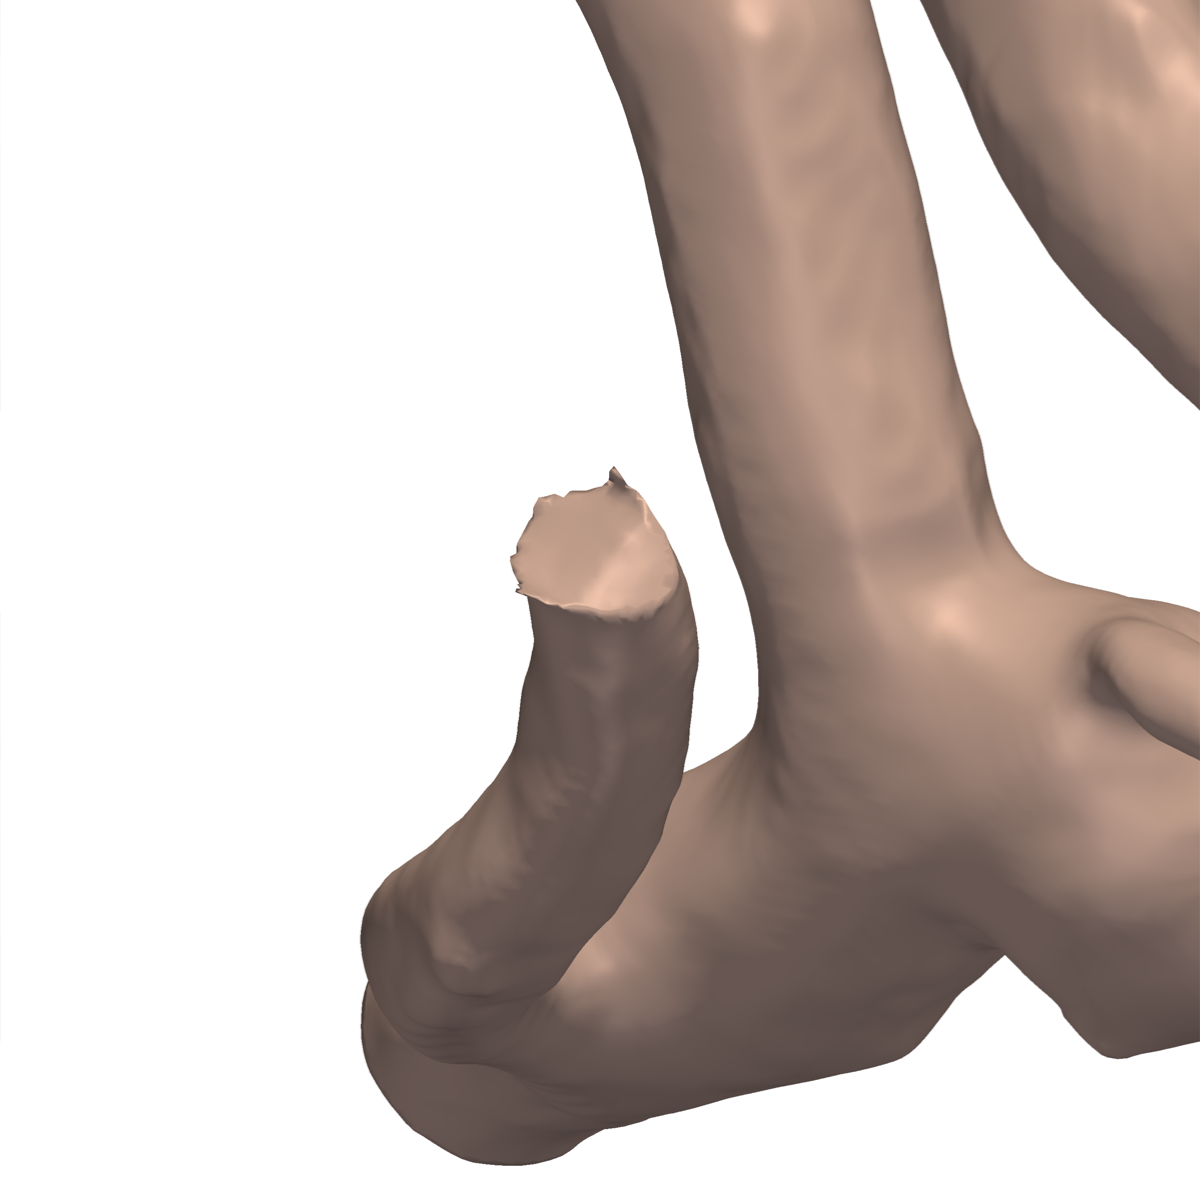
\includegraphics[width=\textwidth]{figures/uncap_USFD54_before.png}\\[-1mm]
        {\footnotesize (a) as published (capped)}
    \end{minipage}\hfill
    \begin{minipage}{0.49\textwidth}\centering
        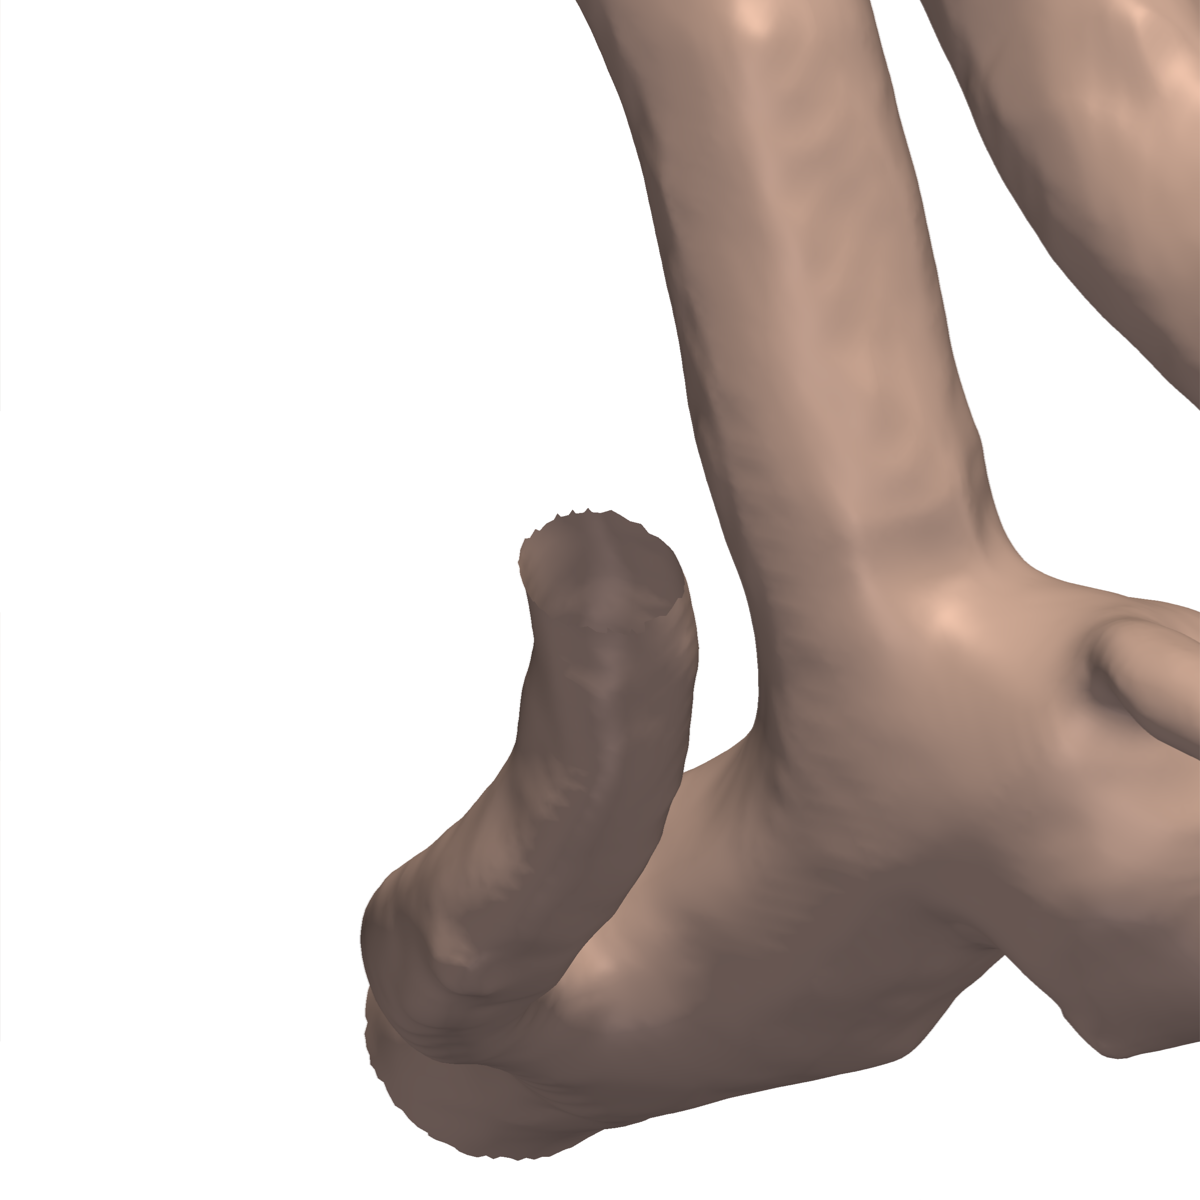
\includegraphics[width=\textwidth]{figures/uncap_USFD54_after.png}\\[-1mm]
        {\footnotesize (b) opened by hand}
    \end{minipage}
    \caption{One outlet of a capped vessel before and after manual uncapping, seen obliquely from outside the vessel. The flat, tilted cap on a short side branch (a) is removed so that the branch ends in an open rim (b), through whose lumen the dark interior is visible. The rest of the surface is unchanged.}
    \label{fig:dp_uncap}
\end{figure}

\subsection{Removal of flow extensions}
\label{sec:dp_ext}

A flow extension is a geometrically simple object: a tube of constant radius, aligned with the vessel axis at the outlet and typically several radii long. A native vessel end almost never looks like this, because within a couple of millimetres it bends, tapers or flares into a bifurcation. The extension remover exploits exactly this difference. Figure~\ref{fig:dp_ext} shows a typical vessel from the extended group.

\begin{figure}[H]
    \centering
    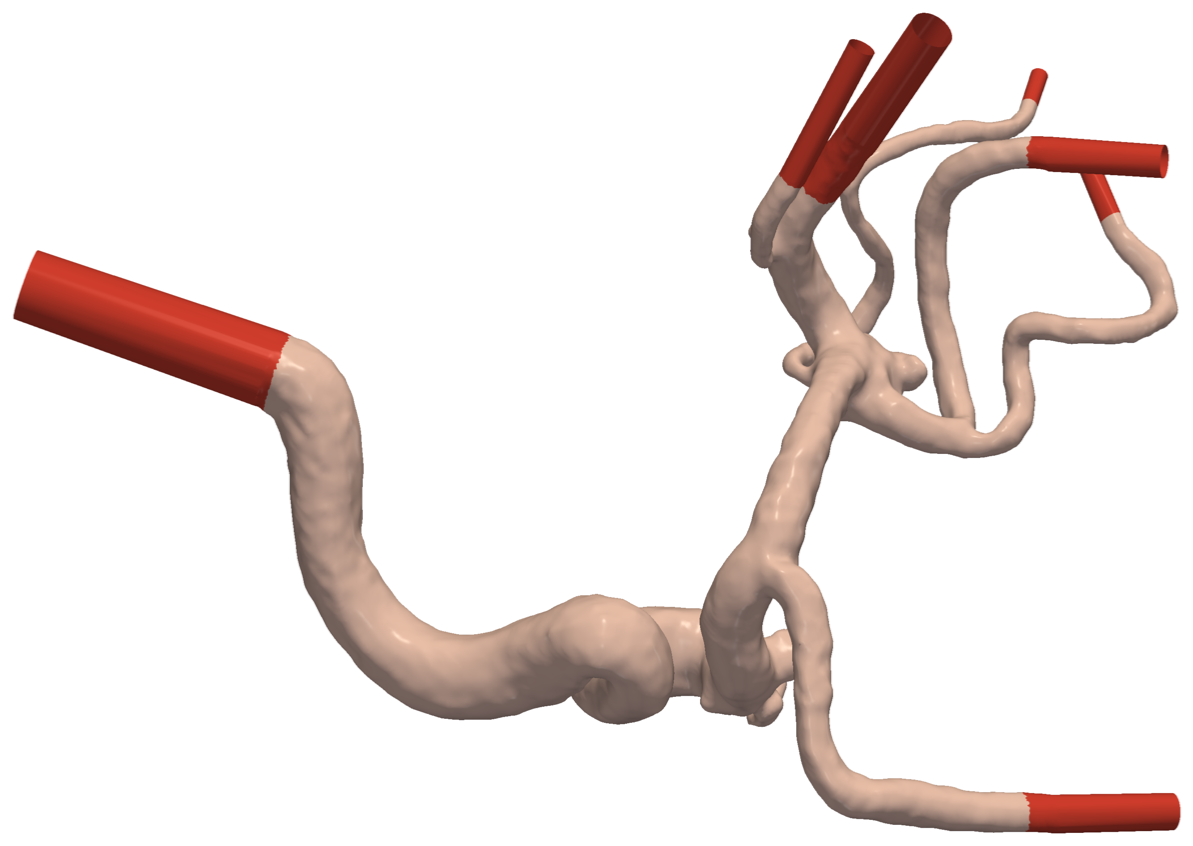
\includegraphics[width=0.78\textwidth]{figures/ext_p398_a.png}
    \caption{A vessel from the extended group with the automatically detected flow extensions highlighted in red. The extensions are perfectly straight, constant-radius tubes; the transition into native anatomy is where the wall starts to tilt, flare or bend.}
    \label{fig:dp_ext}
\end{figure}

For every boundary loop (opening) of the surface we estimate its centroid $\mathbf{c}$, its mean radius $R$ and an axis $\mathbf{a}$ that points into the vessel. Starting from the loop, we then walk into the surface one ring of vertices at a time, much like a breadth-first search on the mesh graph. For the $k$-th ring we measure its axial depth $s_k$, its mean distance from the axis $r_k$, the lateral offset $o_k$ of its centroid from the axis, and the mean absolute alignment $\bar{d}_k = \langle |\mathbf{n}_i \cdot \mathbf{a}| \rangle$ between the vertex normals and the axis. The ring is accepted as still belonging to a cylinder when
\begin{equation}
    |r_k - R| \le 0.18\,R, \qquad \bar{d}_k \le 0.22, \qquad o_k \le 0.35\,R ,
    \label{eq:dp_cyl}
\end{equation}
that is, when its radius has not drifted, the wall is still parallel to the axis, and the ring is still centred on it. The walk stops at the first ring that violates (\ref{eq:dp_cyl}) twice in a row. It also stops at the first sign of a native ostium, which is a radius that flares by more than 8\%, or a wall that starts to tilt while the ring thins. The depth reached is the candidate extension length $L$. An opening is classified as extended only when
\begin{equation}
    L \ge \max\left(1.5\ \text{mm},\; 2R\right),
\end{equation}
which is short enough to catch extensions on 2\,mm perforators yet long enough that a merely straight stretch of native vessel is not mistaken for one.

Each detected extension is then removed with a planar cut perpendicular to its axis. The cut is restricted to a cylinder of radius $1.3R$ around the axis, so that a neighbouring vessel crossing the cutting plane is left untouched. When such a local cut is not accepted, the clipping radius is widened step by step to $1.8R$, $2.2R$ and $3.0R$. A cut is accepted only if it removes the extension and nothing else. Specifically, the number of boundary loops must stay the same, so that no vessel is closed or torn open, and the remaining surface must keep at least 40\% of its vertices. If no clipping radius gives an acceptable cut, the cut is moved back towards the outlet in steps of 6--30\% of $L$. We deliberately leave a short cuff of $\max(0.8\ \text{mm},\ 0.3R)$ of the cylinder in place, because the last millimetre before the detected transition already belongs to the native ostium more often than not. After the cut, the cylinder walk is repeated on the new opening, and a second cut is made if the leftover is still longer than $\max(1.4\ \text{mm},\ 0.7R)$. Finally, the new rim is relaxed with five iterations of Laplacian smoothing along the boundary only (factor 0.5), which removes the sawtooth left by clipping triangles.

Out of the 316 vessels in the extended group, 315 contained at least one extension that met the criteria. Altogether 2388 cuts were made, a median of 8 per vessel and at most 13. The removed lengths had a median of 5.0\,mm and a 5--95\% range of 1.5--13.5\,mm. Every output passed the integrity checks, so no vessel in this group needed manual treatment.

\subsection{Isolation of a single aneurysm}
\label{sec:dp_keepone}

A considerable fraction of patients with an intracranial aneurysm have more than one \citep{juvela2000}, and the database reflects this: 54 of its vessels carry two or more aneurysms. We keep these vessels because they are a valuable source of geometric variety. Our model, however, is built around a single aneurysm per sample, and its template has one sac (Section~\ref{sec:dp_template}). We therefore turn every vessel with $k$ aneurysms into $k$ samples. Each sample keeps one aneurysm, and the other $k-1$ are removed and the parent artery is reconstructed in their place (Figure~\ref{fig:dp_keepone}). In the final set, 54 multi-aneurysm vessels yield 117 single-aneurysm samples, 62 of them at a bifurcation and 55 on a sidewall.

\begin{figure}[H]
    \centering
    \begin{minipage}{0.49\textwidth}\centering
        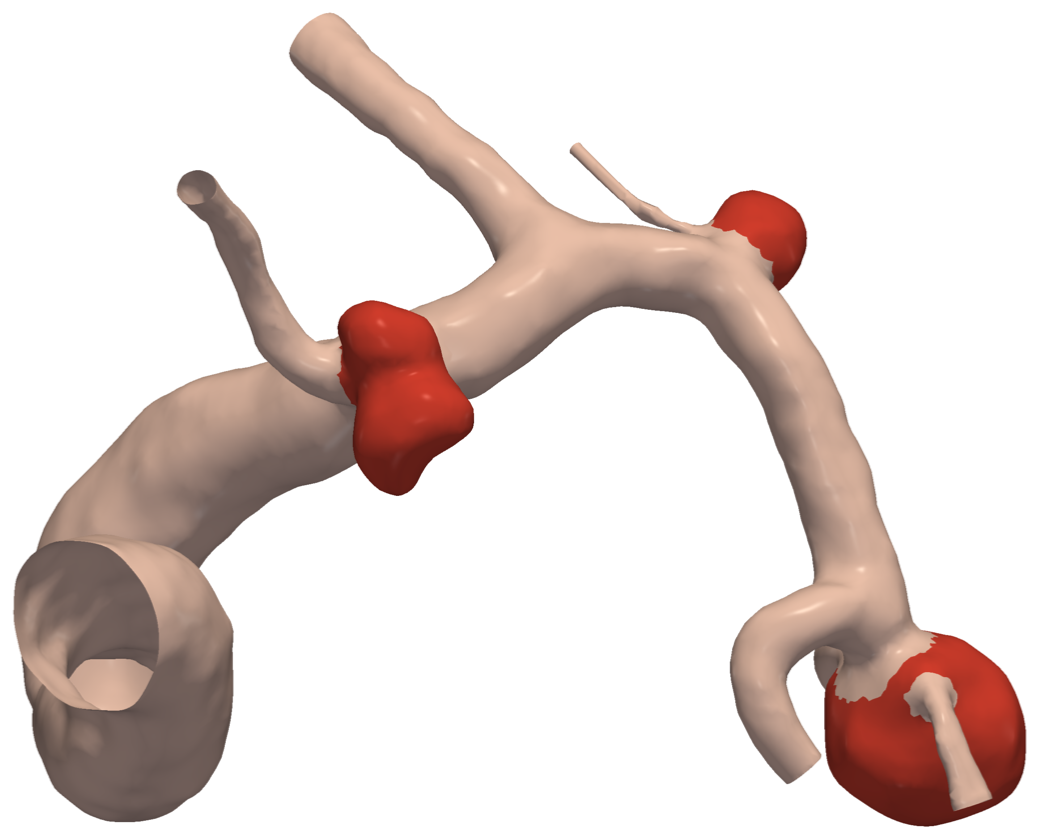
\includegraphics[width=\textwidth]{figures/ko_p305__in.png}\\[-1mm]
        {\footnotesize (a) input}
    \end{minipage}\hfill
    \begin{minipage}{0.49\textwidth}\centering
        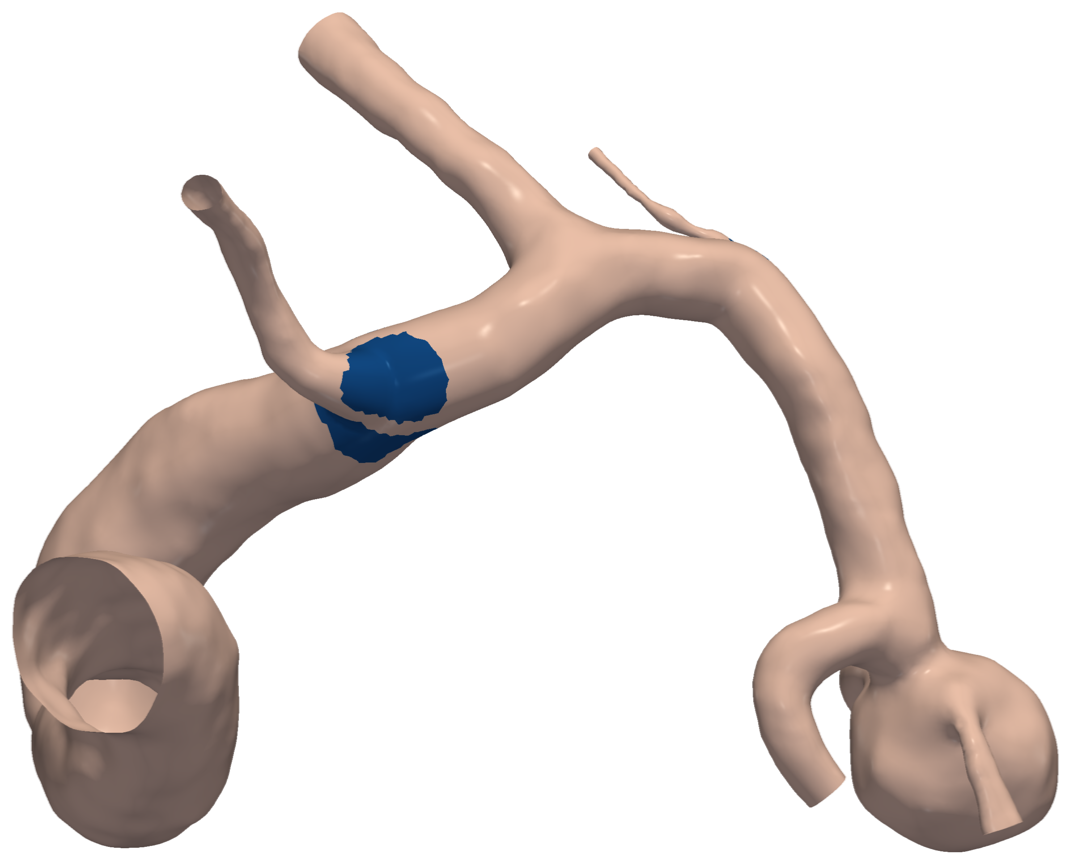
\includegraphics[width=\textwidth]{figures/ko_p305__1_out.png}\\[-1mm]
        {\footnotesize (b) sample 1}
    \end{minipage}\\[2mm]
    \begin{minipage}{0.49\textwidth}\centering
        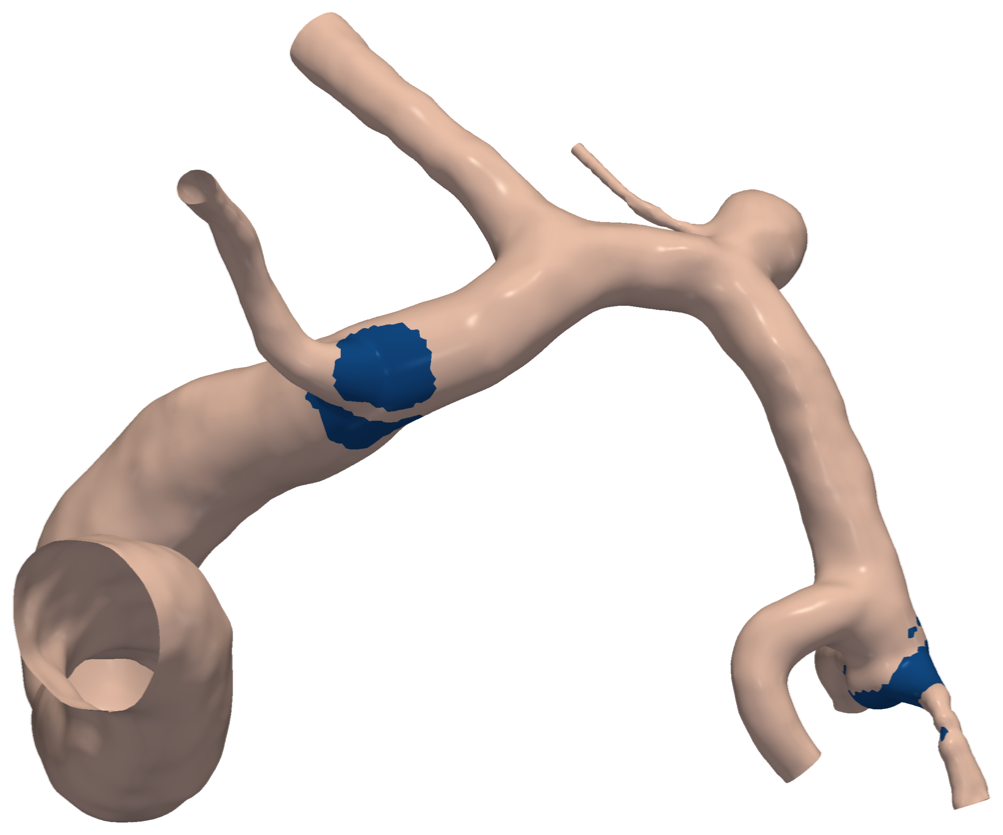
\includegraphics[width=\textwidth]{figures/ko_p305__2_out.png}\\[-1mm]
        {\footnotesize (c) sample 2}
    \end{minipage}\hfill
    \begin{minipage}{0.49\textwidth}\centering
        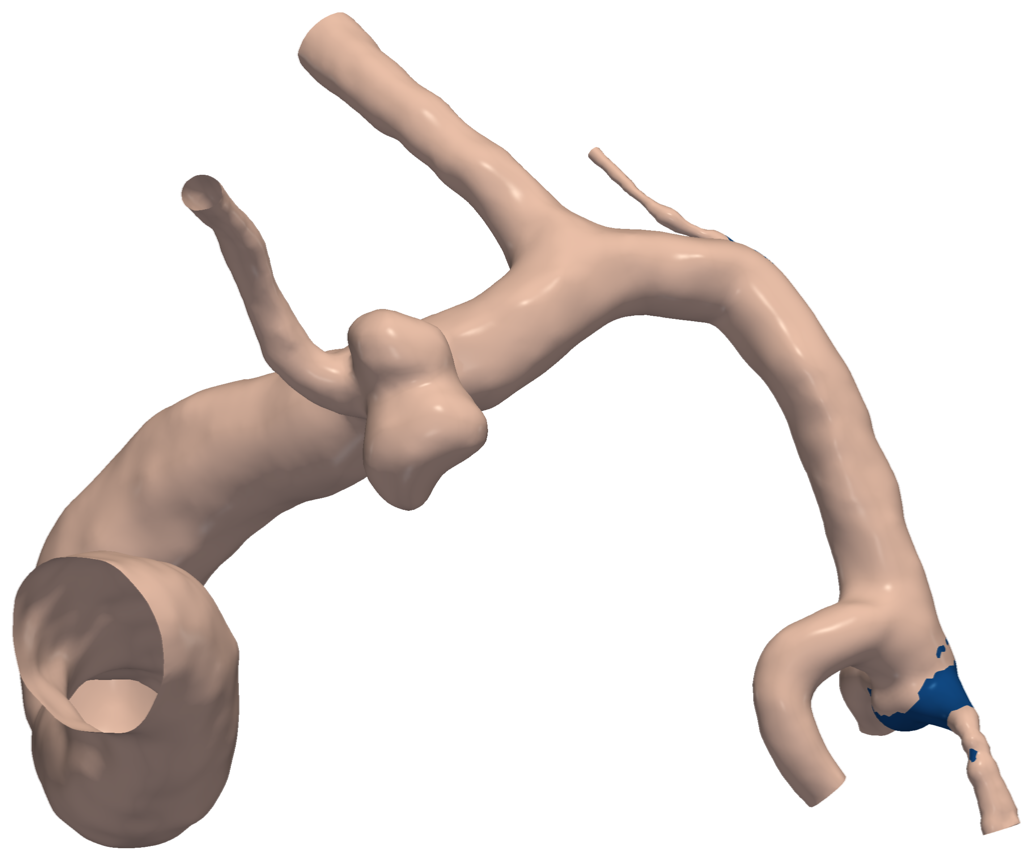
\includegraphics[width=\textwidth]{figures/ko_p305__3_out.png}\\[-1mm]
        {\footnotesize (d) sample 3}
    \end{minipage}
    \caption{Single-aneurysm isolation on a vessel with three aneurysms. (a) The input with all three sacs highlighted in red. (b--d) The three samples generated from it. Each keeps one aneurysm untouched; the wall reconstructed in place of the other two is shown in blue. Everywhere else the sample is identical to the input.}
    \label{fig:dp_keepone}
\end{figure}

The removal follows the Voronoi-based approach of \citet{ford2009}, as implemented in VMTK and formalised by \citet{piccinelli2009}. A tubular surface is described by its internal Voronoi diagram, the centres and radii of the maximal balls inscribed in the lumen. The union of these balls reproduces the lumen, and their centres approximate its medial axis \citep{amenta2001}. An aneurysm appears in this description as a cluster of balls hanging off the parent artery's medial axis. Removing it therefore amounts to removing those balls and filling the gap with balls interpolated from the healthy parent on either side.

\subsubsection*{Seeds and parent centrelines}

For each aneurysm a user places a small number of seed points through a picking interface. Every aneurysm receives a seed on the parent inflow and one on the top of the sac. A sidewall aneurysm additionally receives one seed on the parent downstream of the sac, and a bifurcation aneurysm one on each of the two daughter branches. This is the only manual input to the removal. From the seeds we compute the parent centrelines that run past the aneurysm, using the Voronoi-based method of \citet{antiga2004}, together with the centreline into the sac itself.

\subsubsection*{Voronoi reconstruction of the parent artery}

The Voronoi diagram of the whole vessel is computed once. The Delaunay step occasionally returns a degenerate tetrahedron whose circumsphere is hundreds of millimetres wide and centred far outside the vessel. Such a ball cannot be inscribed in the lumen, and left in the diagram it fills half of space during the reconstruction. We therefore discard every ball wider than the diagonal of the vessel's bounding box. For every aneurysm to be removed, the parent centrelines are cut at the neck and re-interpolated across it. In the region of the neck, only the Voronoi balls lying within a tube of twice the local radius around the healthy parent centreline are kept, and the balls of the sac are discarded. The gap is then filled with the parent's own balls from either side, which are interpolated across it and parallel-transported along the patched centreline \citep{ford2009}. Any remaining ball that still protrudes towards the sac is pruned. The reconstructed lumen is the envelope of the remaining balls (Figure~\ref{fig:dp_voronoi}). We evaluate it as an implicit polyball function on a 0.1\,mm grid and extract its surface with marching cubes \citep{lorensen1987}.

\begin{figure}[H]
    \centering
    \begin{minipage}{0.49\textwidth}\centering
        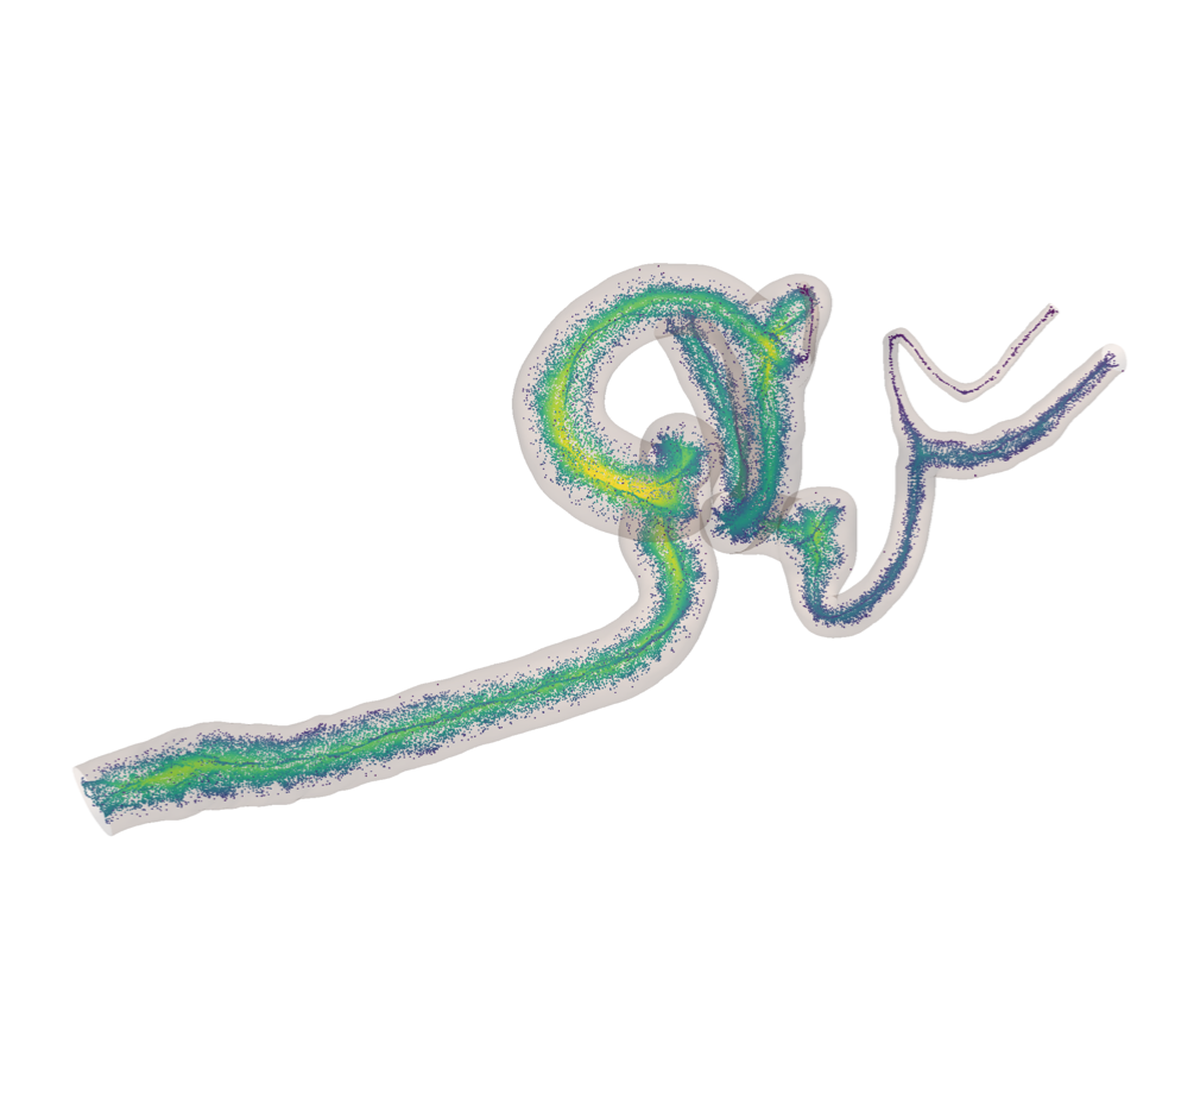
\includegraphics[width=\textwidth]{figures/vor_a.png}\\[-1mm]
        {\footnotesize (a) Voronoi diagram of the vessel}
    \end{minipage}\hfill
    \begin{minipage}{0.49\textwidth}\centering
        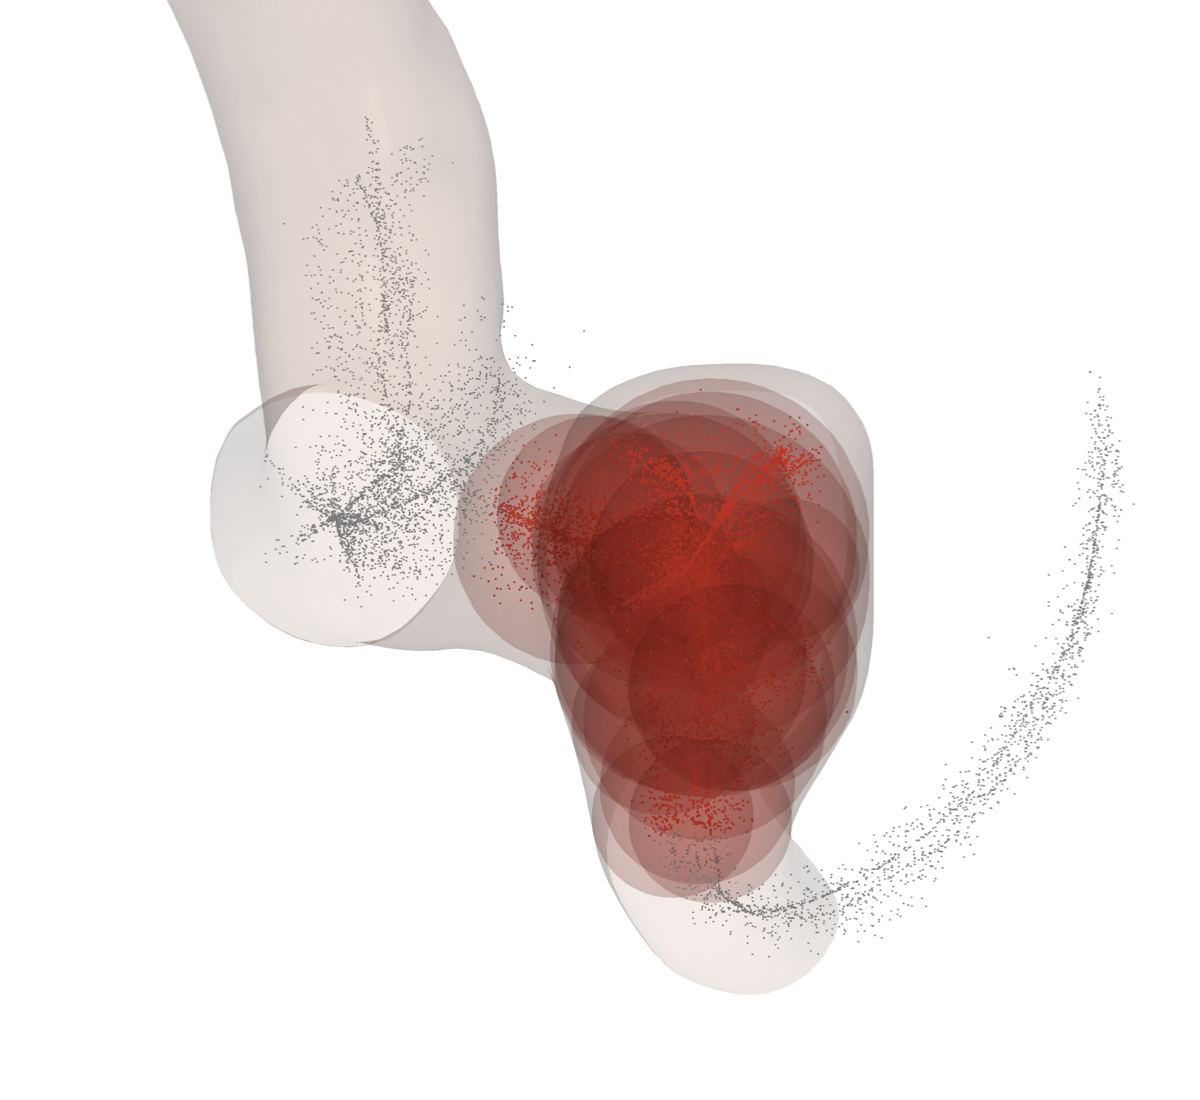
\includegraphics[width=\textwidth]{figures/vor_b.png}\\[-1mm]
        {\footnotesize (b) balls of the sac}
    \end{minipage}\\[2mm]
    \begin{minipage}{0.49\textwidth}\centering
        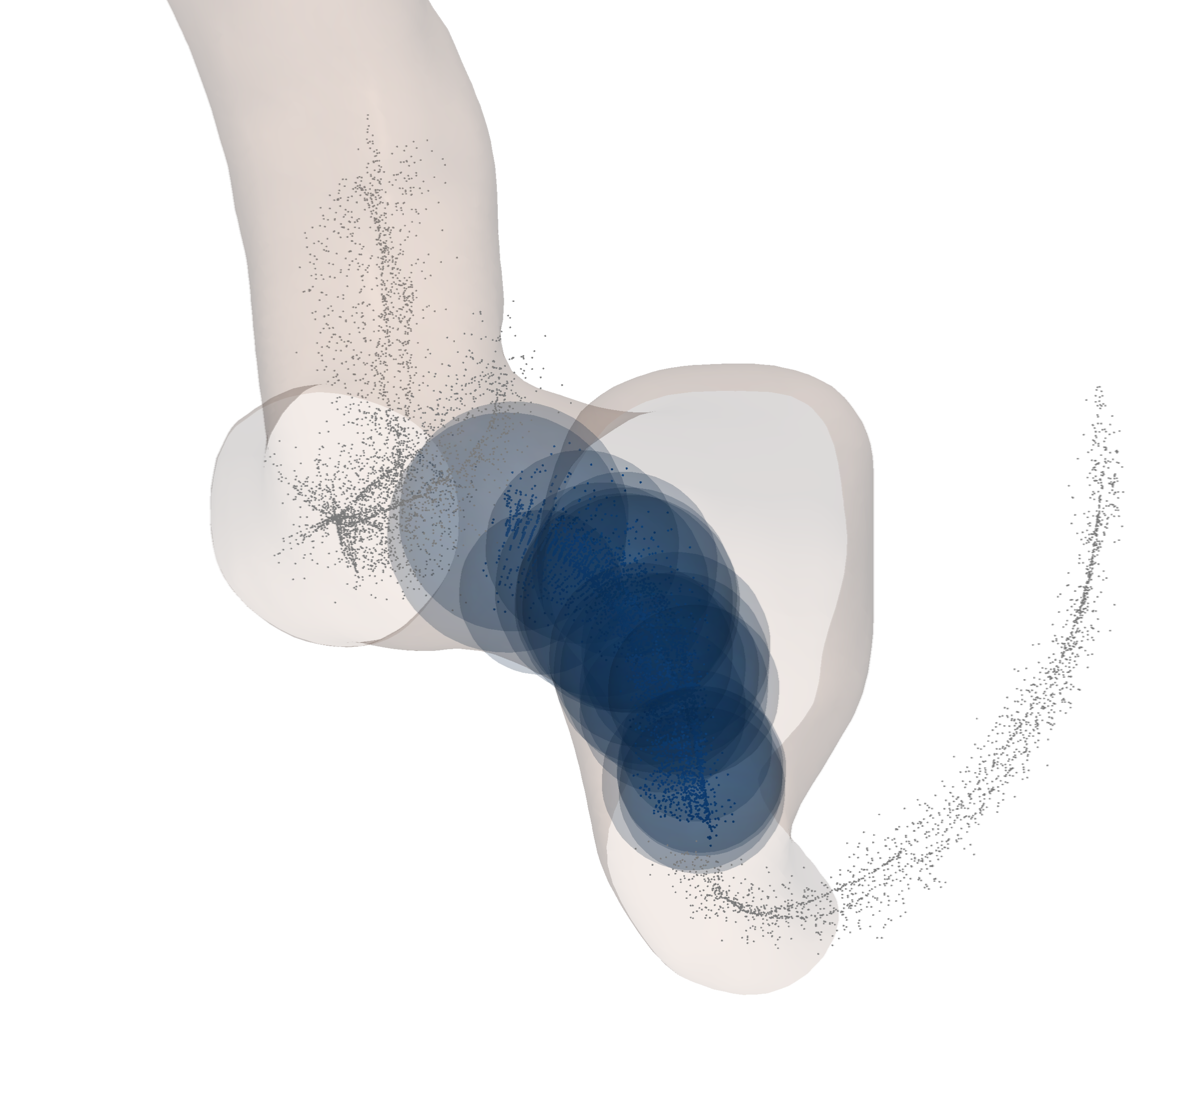
\includegraphics[width=\textwidth]{figures/vor_c.png}\\[-1mm]
        {\footnotesize (c) balls interpolated from the parent}
    \end{minipage}\hfill
    \begin{minipage}{0.49\textwidth}\centering
        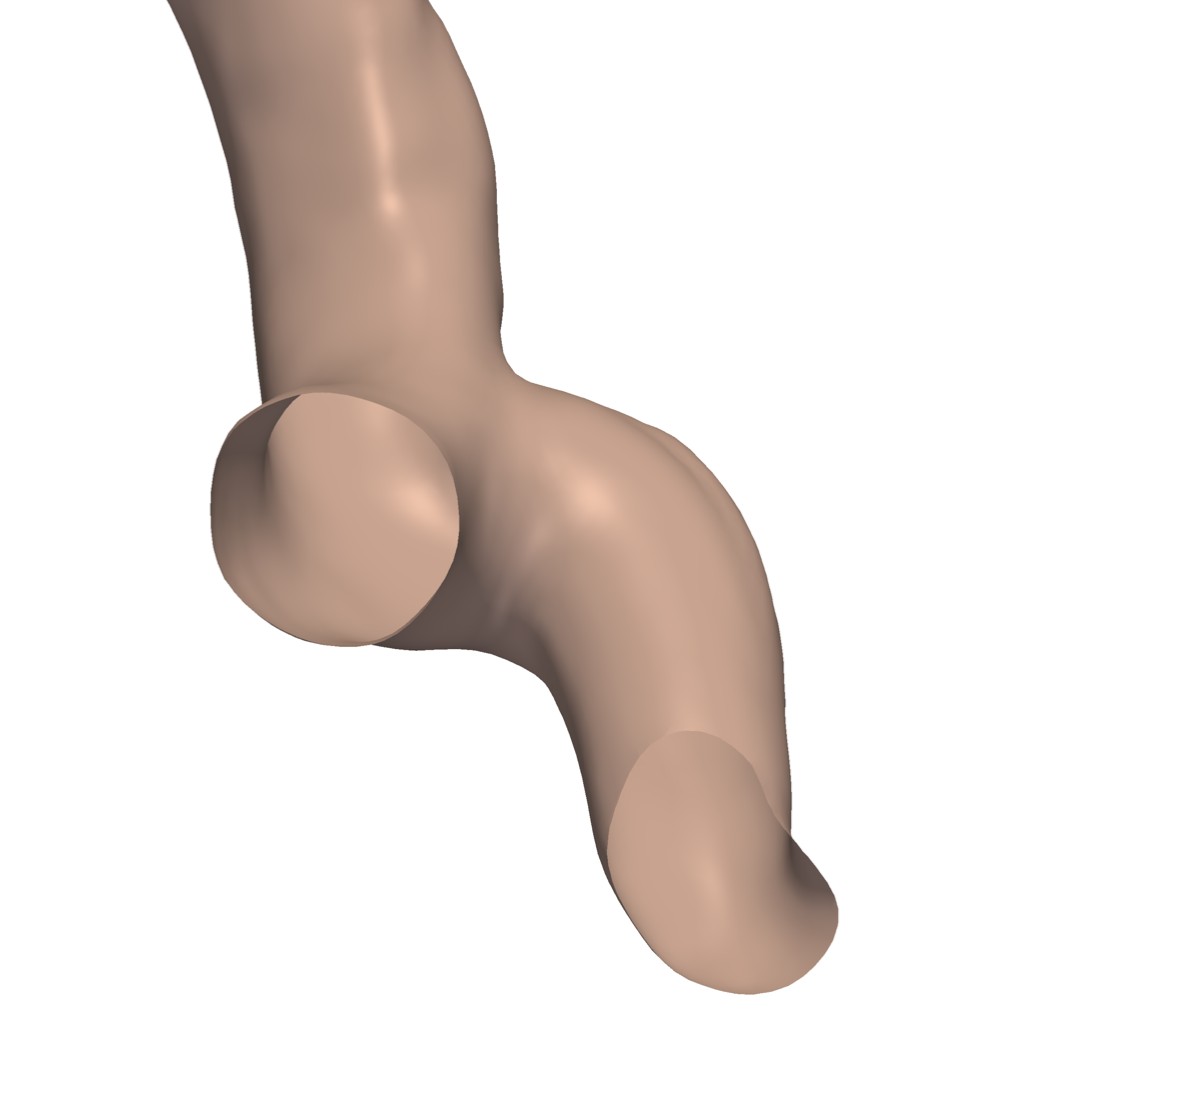
\includegraphics[width=\textwidth]{figures/vor_d.png}\\[-1mm]
        {\footnotesize (d) reconstructed lumen}
    \end{minipage}
    \caption{Removal of an aneurysm in the Voronoi description. (a) The centres of the maximal inscribed balls of a vessel, coloured by radius (blue small, yellow large), inside the ghosted wall. The balls cluster along the medial axis. (b) Around one aneurysm, the balls of the sac (red, centres and a sample of the balls themselves) hang off the balls of the parent artery (grey centres). (c) The sac balls are discarded and balls interpolated from the parent on either side (navy) take their place. (d) The envelope of the remaining balls is the reconstructed lumen, extracted by marching cubes. In (b--d) the part of the vessel in front of the neck is cut away for visibility.}
    \label{fig:dp_voronoi}
\end{figure}

\subsubsection*{Grafting back onto the original wall}

A surface extracted from a voxel grid loses the fine texture of the original wall, and that texture is exactly what the network is supposed to learn. We therefore keep the reconstructed surface only where the anatomy actually changed. Every vertex of the reconstruction that lies within a small distance of the original wall is snapped back onto it. The seam between the snapped and the reconstructed part is faired with a biharmonic (thin-plate) energy \citep{botsch2008}, so that the reconstructed patch joins the original wall without a visible kink. The openings of the vessel are restored by clipping the result at the original opening planes. Finally, the surface is remeshed with its boundary held fixed. As Figure~\ref{fig:dp_keepone} shows, the reconstruction (blue) is confined to the region of the removed sac and its immediate surroundings.

\subsubsection*{Quality gates and retries}

Removing a sac at a crowded bifurcation can go wrong in characteristic ways. The interpolated parent can seal a neighbouring branch. It can split the lumen into two thin volumes. It can leave a residual pocket where the sac used to be. Or it can produce a surface with a handle where two reconstructed walls touch. Each sample therefore passes a set of gates. The number of openings must equal that of the input, which rules out a sealed or torn branch. The lumen must remain one connected volume with no enclosed pockets. The surface must be a single manifold component of genus zero without fan-shaped artefacts. Finally, no part of the removed sac may survive more than 0.25\,mm off the reconstructed parent. When a gate fails, the removal is retried with adjusted clipping of the parent centrelines, up to six times. A sample that still fails is rejected. All 117 samples passed. They were also inspected visually, one by one, and accepted.

\subsubsection*{Assembly of the dataset}

The final set is assembled from the outputs of the previous steps with a fixed priority. A single-aneurysm sample takes precedence over the vessel it was derived from. A hand-uncapped or automatically unextended surface takes precedence over the original. An untouched original is used only when no processed version exists. One patient (three vessels) was excluded from the dataset after visual review. Five pairs of vessels in the database turned out to be the same patient scanned in the same frame, with more than 95\% volumetric overlap. In these cases the database already provides one model per aneurysm, so our single-aneurysm samples replaced them instead of duplicating them. The assembled set contains 737 surfaces: 117 from aneurysm isolation, 387 from cap or extension removal and 233 used as published.

\subsection{Uniform remeshing of the ground truth}
\label{sec:dp_remesh}

The assembled surfaces are anatomically clean, but their triangulation is not suitable as a training target. The meshes were generated for CFD and morphometry with area-based element sizes. Edge lengths differ between vessels and within a single vessel, and sub-micrometre edges are common. On the example vessel used in the figures of this section, edges range from 2\,$\mu$m to more than twice the mean, with a coefficient of variation (CV) of 0.25. A network that compares a predicted surface with such a target in effect weights the loss by the local vertex density, which is an artefact of the segmentation software rather than a property of the anatomy. The GT is therefore remeshed to a single target edge length of 0.15\,mm. Across the assembled surfaces the mean edge length ranges from 0.11 to 0.33\,mm (5--95\%, median 0.20\,mm). We chose the target at the fine end of this range, so that remeshing does not noticeably coarsen any surface and the finest-resolved vessels keep their detail. Three requirements guided this stage: the edge length must be uniform across the whole dataset, as little wall texture as possible may be lost to smoothing, and every opening must be a clean pipe section perpendicular to the vessel axis.

\subsubsection*{Openings as pipe sections}

The rims of the source surfaces are wherever the segmentation or the manual uncapping happened to end, which is often oblique and sometimes ragged. We replace each rim with a planar cut perpendicular to the centreline. This gives the network a consistent definition of where a vessel ends, and it lets the template be cut on exactly the same planes later on (Section~\ref{sec:dp_template}). For every opening we define an \emph{ostium frame} $(\mathbf{o}, \mathbf{n}, r)$, consisting of an origin $\mathbf{o}$ at the centroid of the rim, an outward normal $\mathbf{n}$ and a radius $r$. The normal is the mean centreline tangent over an arc of two opening radii (at least 1\,mm) before the opening. It is not allowed to tilt by more than $50^\circ$ from the normal of the rim's own best-fit plane. If the centreline does not actually reach the opening, which happens for very small side branches, the rim normal is used instead. The centreline used for the frames is computed on a disposable working copy of the surface, which is decimated and strongly smoothed so that the Voronoi diagram can be built robustly. The working copy is discarded afterwards, and only the frames are carried forward.

An oblique rim cannot simply be cut by a perpendicular plane through its centre, because part of the wall falls short of the plane. We therefore first append a temporary 5\,mm flow extension to every opening \citep{antiga2008}. The perpendicular plane then cuts through a complete tube. The cut itself is limited to a cylinder of $\max(1.5r,\ r + 0.2\ \text{mm})$ around the axis, so that a neighbouring vessel passing near the plane is not affected. After the cut, the extension has disappeared and the rim lies exactly on the frame's plane. The frames are stored next to the GT, since the centreline and template stages both consume them.

\subsubsection*{Isotropic remeshing}

The cut surface receives a single light pass of Taubin smoothing \citep{taubin1995,taubin1996}. We use five iterations of the windowed-sinc low-pass filter with a weak pass band, which removes the clipping facets but leaves the wall texture in place. The surface is then remeshed with VMTK's isotropic remesher, which alternates edge splits, collapses and flips with tangential relaxation \citep{botsch2004,botsch2010}. We found that more remeshing iterations do not help on these surfaces. The tangential relaxation oscillates instead of converging, and on one vessel 20 iterations grew the surface area more than fivefold. Six iterations with ten connectivity passes preserved the area, the texture and the edge-length uniformity best, and also ran about three times faster.

The remesher is sensitive to near-coincident vertices in its input, which the source data contains plenty of. Every remesh is therefore verified. If the area drifts by more than 15\% or the surface stops being manifold, the input is welded at a progressively larger tolerance (0.05 to 0.25\,mm) and the remesh is repeated. A final clean-up removes the few remaining needle triangles, enforces a minimum edge length and orients all faces outwards. Before it is saved, each GT has to pass two gates. Its area must lie within 0.88--1.20 times that of the source, which catches both a lost sac or branch and an extension that was not clipped off. It must also have exactly as many openings as the source, since a torn rim would show up as an additional one. An audit of the final set further confirmed that every GT is a single manifold component of genus zero with exactly one planar rim per ostium frame.

\begin{figure}[H]
    \centering
    \begin{minipage}{0.49\textwidth}\centering
        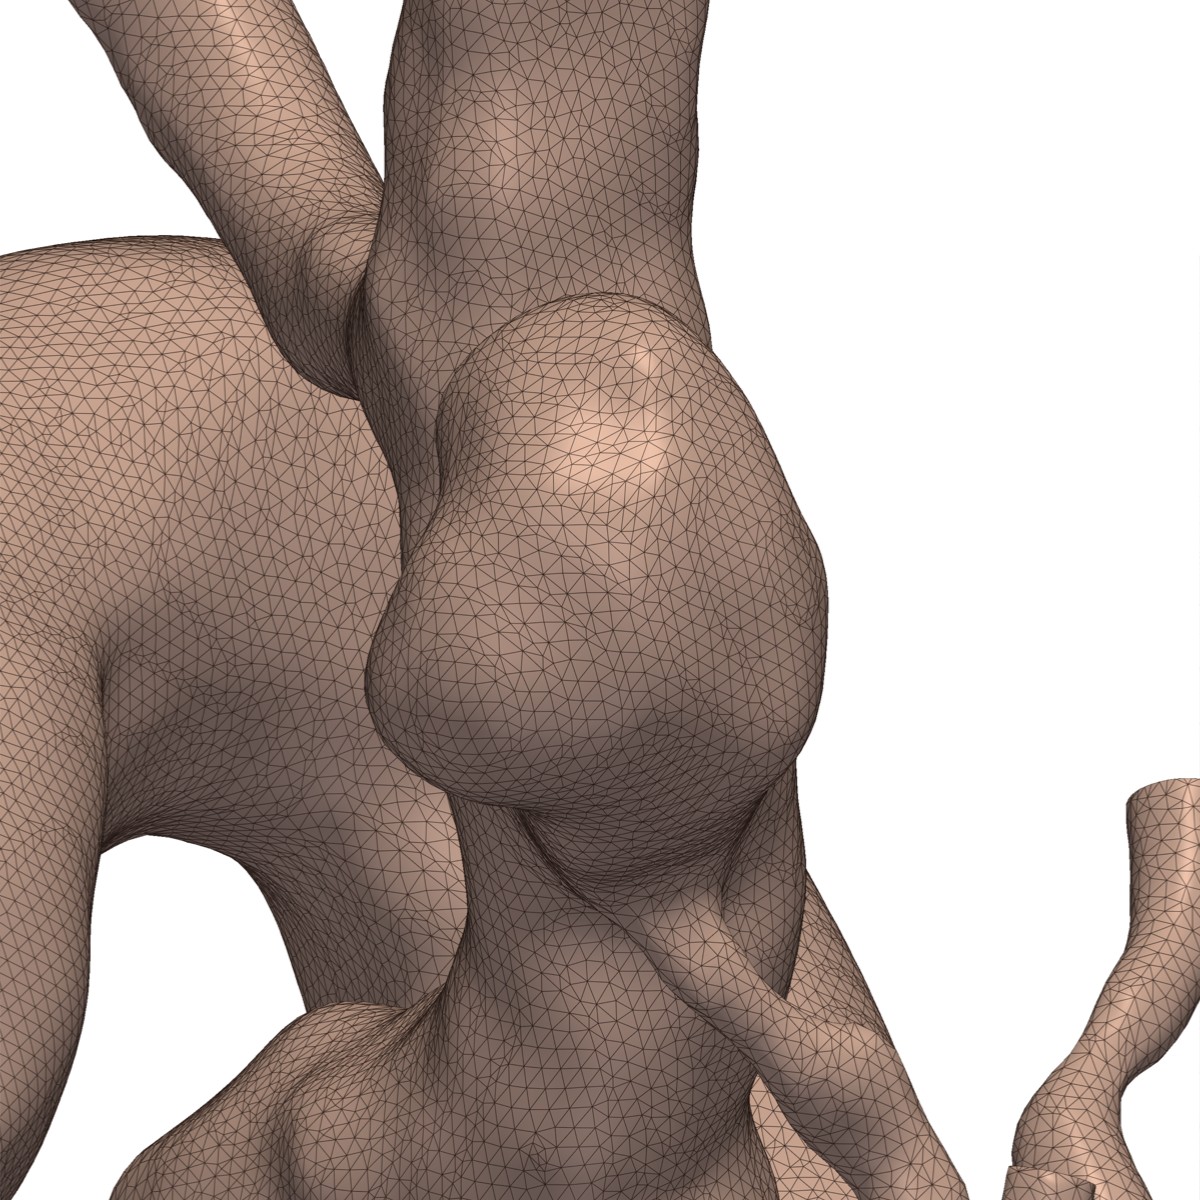
\includegraphics[width=\textwidth]{figures/rem_p141_sac_src.png}\\[-1mm]
        {\footnotesize (a) source, sac}
    \end{minipage}\hfill
    \begin{minipage}{0.49\textwidth}\centering
        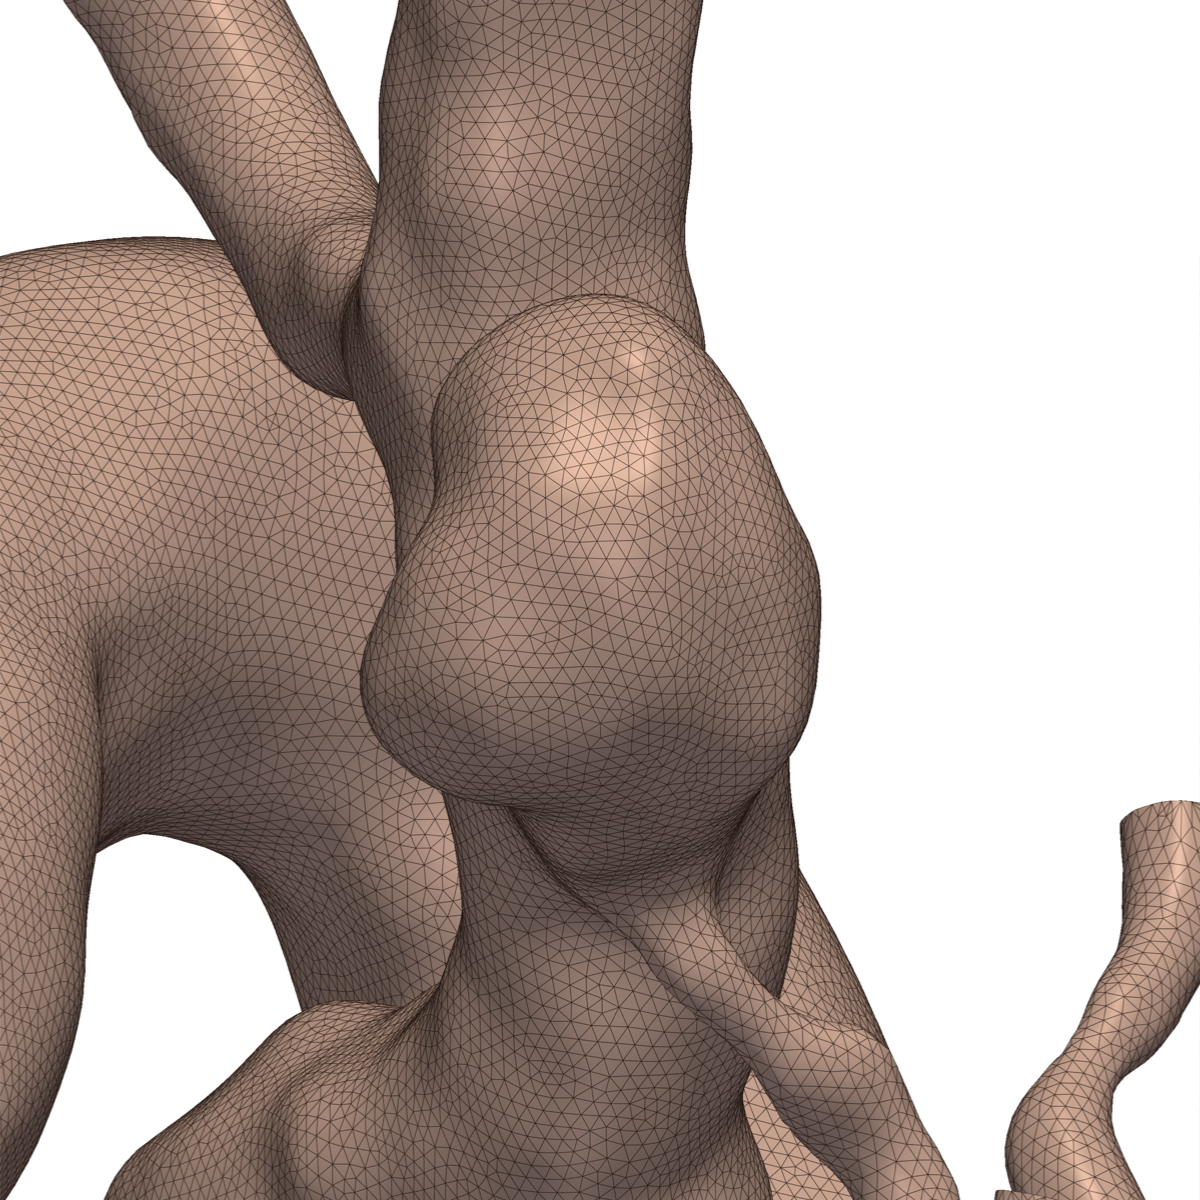
\includegraphics[width=\textwidth]{figures/rem_p141_sac_uni.png}\\[-1mm]
        {\footnotesize (b) uniform GT, sac}
    \end{minipage}\\[2mm]
    \begin{minipage}{0.49\textwidth}\centering
        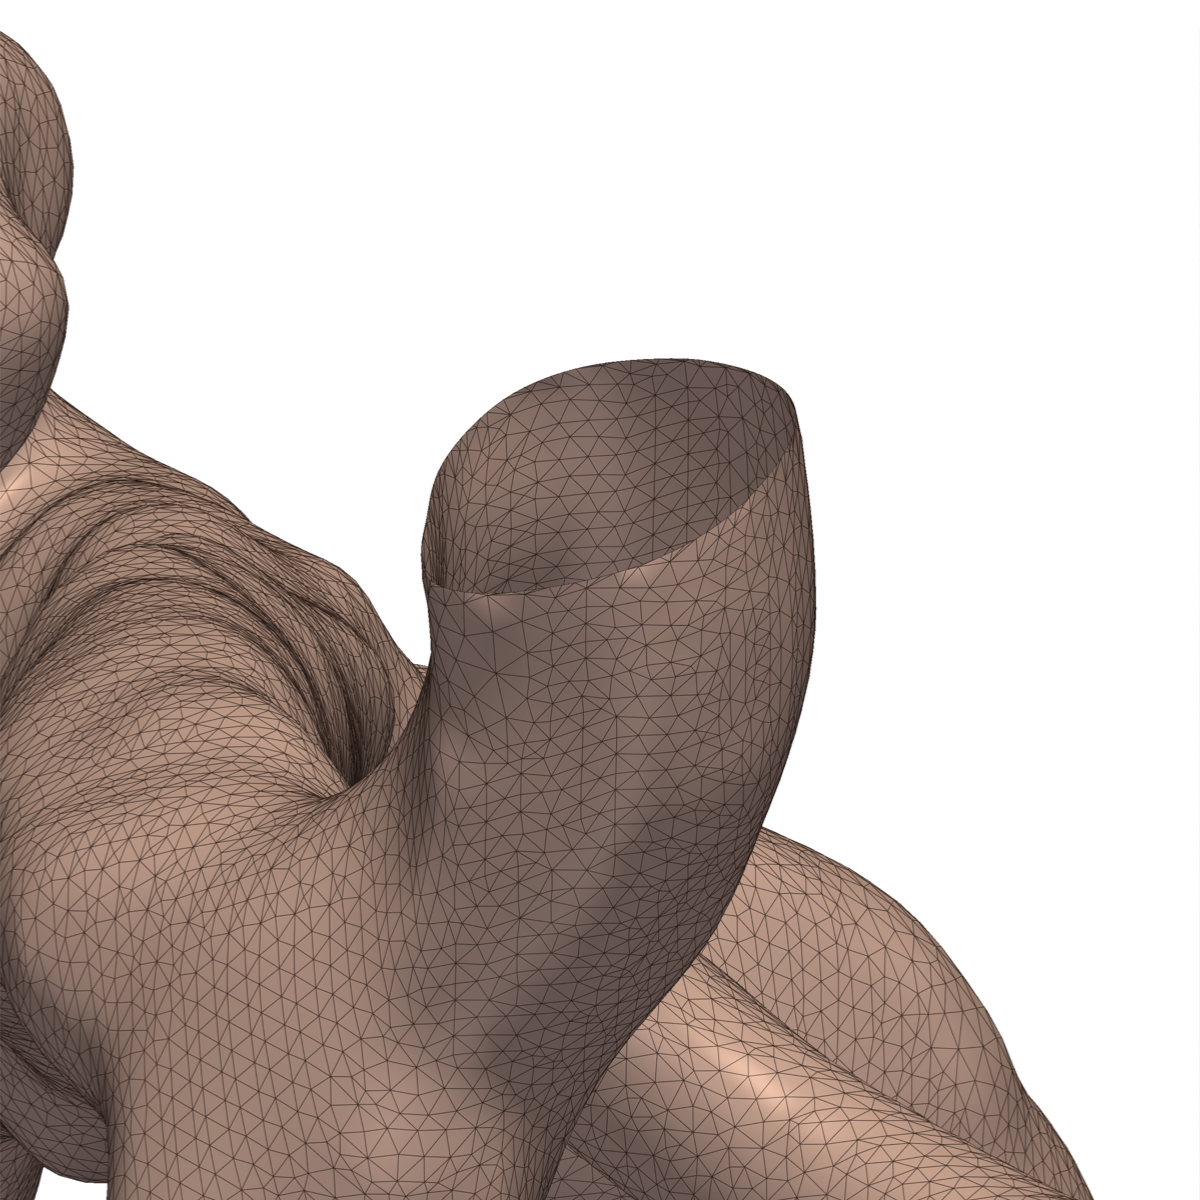
\includegraphics[width=\textwidth]{figures/rem_p141_ost_src.png}\\[-1mm]
        {\footnotesize (c) source, opening}
    \end{minipage}\hfill
    \begin{minipage}{0.49\textwidth}\centering
        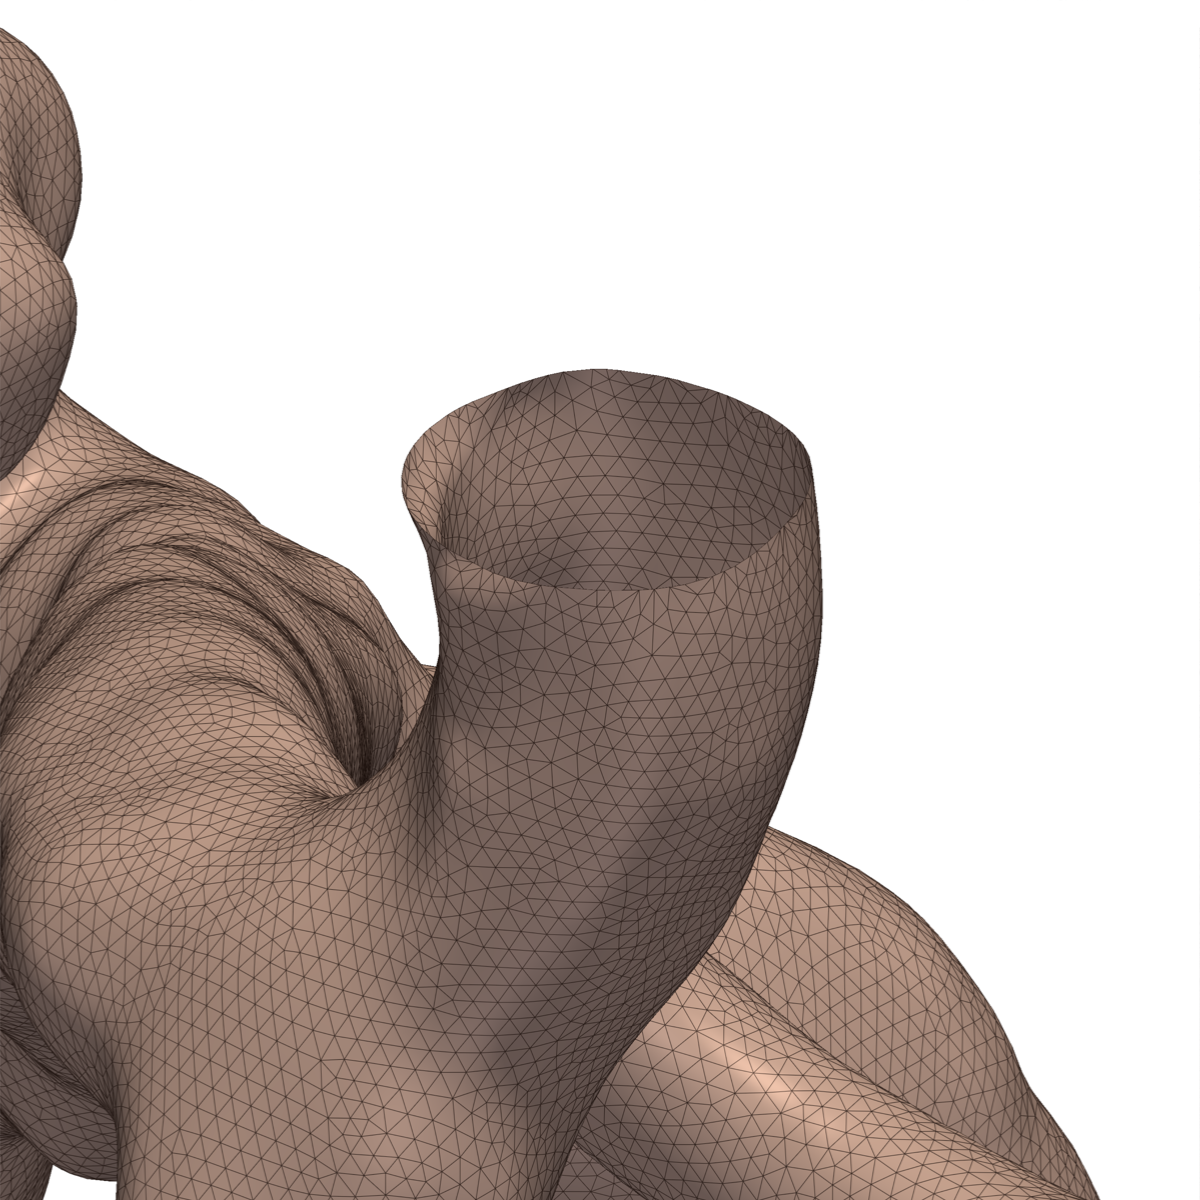
\includegraphics[width=\textwidth]{figures/rem_p141_ost_uni.png}\\[-1mm]
        {\footnotesize (d) uniform GT, opening}
    \end{minipage}
    \caption{Uniform remeshing. (a, b) The aneurysm sac before and after remeshing: the triangle size becomes uniform (edge-length CV 0.25 $\rightarrow$ 0.12, shortest edge 2\,$\mu$m $\rightarrow$ 24\,$\mu$m) while the shape and texture of the wall are preserved. (c, d) An opening before and after, seen obliquely from outside the vessel: the uneven rim is replaced by a planar pipe-section cut perpendicular to the centreline.}
    \label{fig:dp_remesh}
\end{figure}

All 737 surfaces passed the gates. Across the dataset, the remeshed GT has a mean edge length of 0.124\,mm (the remesher settles slightly below its target), with the per-surface means lying within 0.123--0.124\,mm (5--95\%), and a median shortest edge of 25\,$\mu$m instead of 6\,$\mu$m. Its median within-surface edge-length CV is 0.13, compared with 0.22 for the source surfaces (Figure~\ref{fig:dp_edges}), and its area is 0.99 times that of the source (1--99\%: 0.98--0.99), so the remesh and the rim cuts change the surface only marginally. The GT surfaces have a median of 102\,987 vertices (5--95\%: 52\,096--167\,982) and between 2 and 15 openings (median 5).

\begin{figure}[H]
    \centering
    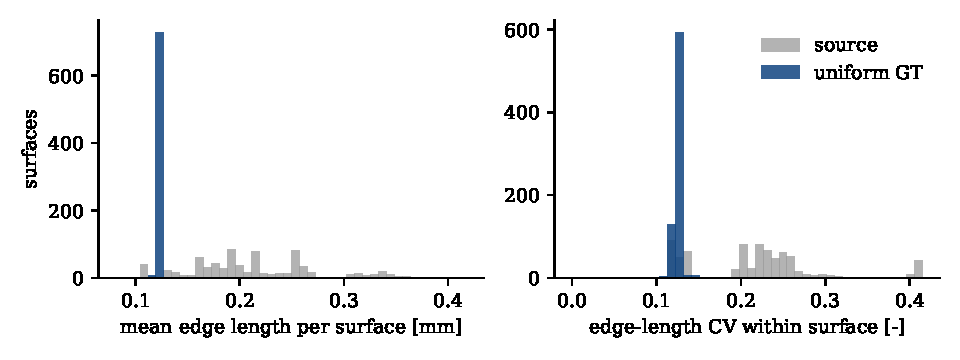
\includegraphics[width=0.95\textwidth]{figures/edge_stats.pdf}
    \caption{Edge-length statistics over the whole dataset, before (grey) and after (blue) uniform remeshing. Left: mean edge length per surface. Right: within-surface coefficient of variation of the edge length (the last source bin collects all values above it). Remeshing collapses the spread between surfaces and reduces the spread within them from a median CV of 0.22 to 0.13.}
    \label{fig:dp_edges}
\end{figure}

\subsection{Centreline extraction}
\label{sec:dp_centreline}

The centreline is the backbone of the two-stage model. The first stage will produce it, and the template is built from it. Following the Introduction, we use the centreline because it averages the wall radially and is therefore robust to segmentation noise, and because together with the maximal inscribed sphere radius (MISR) it is a compact and complete description of a tubular structure \citep{antiga2004,piccinelli2009,sangalli2009}.

We compute centrelines with VMTK, which traces them as minimal paths through the Voronoi diagram of the surface weighted by the inverse of the inscribed radius \citep{antiga2004,antiga2008}. Each path therefore stays as far from the wall as possible, and every point carries its MISR. The input is the uniform GT of Section~\ref{sec:dp_remesh}, so the centreline is consistent with the target the network learns. As before, the Voronoi diagram is built on a working copy of the GT. The copy is cleaned of degenerate triangles and lightly smoothed (Taubin, 15 iterations), since the Voronoi diagram is sensitive to sliver triangles in a way that the network is not. The largest opening is taken as the inlet and every other opening as an outlet. The seeds are placed at the rim centroids, which coincide with the ostium frame origins because the rims are planar.

Two details matter for the quality of the result. First, a Voronoi centreline never quite reaches the opening it is traced to. It stops roughly one radius inside, where the inscribed sphere first touches the rim. We therefore trace the centreline on a copy with 5\,mm temporary extensions and, separately, on the bare surface, and keep whichever trace covers more of the vessel. Each branch end is then extended along its tangent until it meets its ostium plane. Second, Voronoi traces of thin side branches occasionally leave a branch out entirely, especially where a small vessel leaves a large one. We check that every opening is reached by the centreline, and where one is not, we re-trace locally on a refined crop of the surface around that ostium and splice the result into the network.

The traced centreline is resampled at a uniform 0.1\,mm spacing and smoothed with VMTK's centreline smoothing filter while keeping the MISR values. It is then split into branches at the bifurcations with VMTK's branch extractor \citep{antiga2004}. Finally, it is clipped at the ostium planes so that it does not extend past the GT surface. Figure~\ref{fig:dp_centreline} shows the result for the example vessel. The centreline follows each branch from the inlet to every opening, and its colour shows how the MISR tracks the calibre of the vessel. All 737 surfaces produced a centreline that reaches every opening. Across the dataset the centrelines have a median total length of 349\,mm and a median MISR of 1.81\,mm.

\begin{figure}[H]
    \centering
    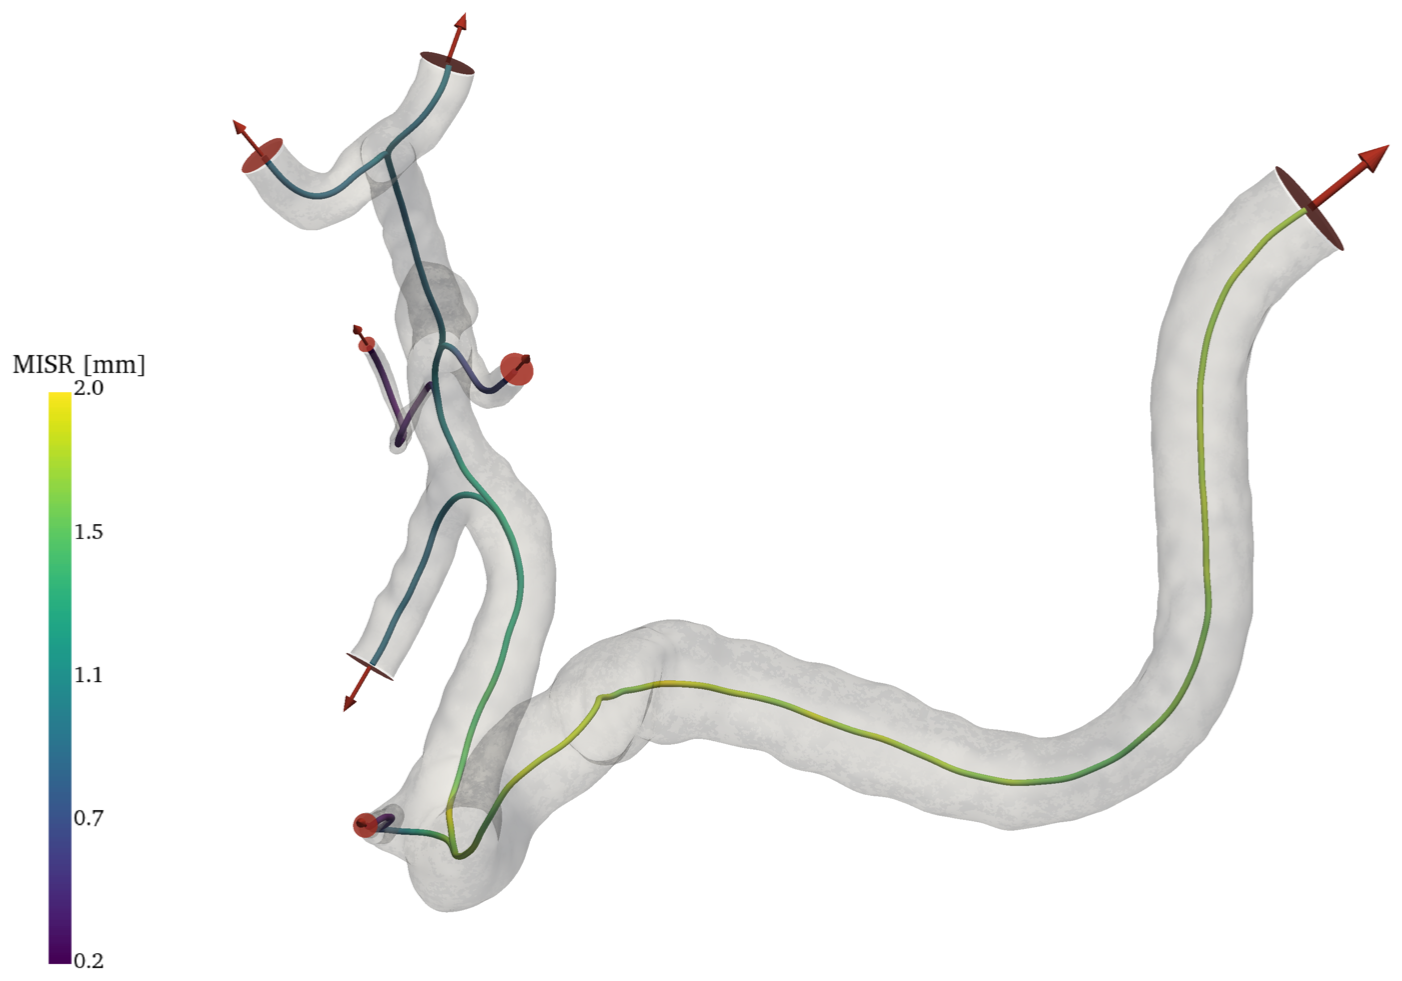
\includegraphics[width=0.80\textwidth]{figures/cl_p141.png}
    \caption{Centreline of the example vessel inside the (translucent) GT surface, coloured by the maximal inscribed sphere radius. The red discs and arrows are the ostium frames: each opening's plane, outward normal and radius. The centreline ends exactly on these planes.}
    \label{fig:dp_centreline}
\end{figure}

\subsection{Template creation}
\label{sec:dp_template}

The template is the coarse surface that stage two deforms into the GT. Its design is dictated by what stage one will eventually be able to produce. The template must be generated from the centreline, its radius, the ostium planes and a small number of parameters for the aneurysm, and from nothing else. If the template were derived from the GT surface itself, the second stage would learn to depend on information that a generative first stage cannot supply. On the other hand, the template should be close enough to the GT that the deformation stage two must learn remains small and smooth. It must also share the GT's topology exactly, with the same openings in the same planes, one connected sac and no handles.

We parametrise the aneurysm with three spheres. Spheres are the simplest primitive whose union can represent both the round sacs and the elongated or multi-lobed sacs found in the data. Three spheres were enough to capture the gross shape of the sacs in our dataset, which keeps the parameter vector short (12 numbers per aneurysm). The template is then the union of a parent tube swept along the centreline and the three spheres, blended into the parent at the aneurysm neck. Building it from the GT takes four steps: detecting the aneurysm, fitting the spheres, building an implicit surface, and meshing it. At inference time only the last two steps are needed. They take the centreline and the sphere parameters as their only inputs.

\subsubsection*{Aneurysm detection}

The aneurysm is detected as the part of the wall that stands off a healthy parent tube. The MISR along the centreline cannot be used directly to describe this tube, because the inscribed sphere swells into the sac at the neck. We therefore apply a morphological opening (an erosion followed by a dilation) to the radius along the centreline graph, with a window of 3.5\,mm. This removes every spike shorter than the window, such as the swelling at a neck, but keeps genuine changes of calibre. The opened radius $\bar{r}$ defines a parent tube $P$, the union of balls $B(\mathbf{u}_j, \bar{r}_j)$ centred on the centreline points $\mathbf{u}_j$. For every wall vertex $\mathbf{x}$ we compute its \emph{excess}
\begin{equation}
    e(\mathbf{x}) = \min_j \left( \lVert \mathbf{x} - \mathbf{u}_j \rVert - \bar{r}_j \right),
\end{equation}
the signed distance by which it stands off the parent tube. The sac is a compact, connected region of high excess. Its dome lies at a local maximum of $e$, and its extent is the connected level set of $e$ around the dome at the lowest level for which the set stays compact. One level lower, the set starts to spill along the parent wall. Several peaks are examined, since a bend of the parent or a cut end can also stand off the tube. Peaks whose regions touch are merged as lobes of one sac. The winning region is the one with the largest volume off the parent relative to its breadth. Peaks close to an open end are discarded as cut-end artefacts. Finally, the detected region is grown by a short geodesic lip of $0.7$ parent radii (clipped to 0.55--1.8\,mm) so that it includes the neck. This is a deliberately simple definition of the neck; for a more elaborate, Voronoi-based alternative see \citet{cardenes2011}.

Not all of the parent artery near the sac plays the same role. The sac grows out of its parent at the neck, but at a crowded bifurcation it often also presses against another stretch of vessel, such as a loop of the same artery or a neighbouring branch. If the template's sac were blended into those as well, it would fuse vessels that are separate in the GT and create a handle. We therefore classify the centreline points near the sac. The \emph{neck} is a short window of centreline from which a straight path into the sac stays inside the lumen. Everything beyond a short buffer around it is \emph{foreign}. The sac will be blended into the neck and kept at a distance from foreign vessel.

\subsubsection*{Sphere fitting}

Let $f_i(\mathbf{x}) = \lVert \mathbf{x} - \mathbf{c}_i \rVert - \rho_i$ be the signed distance to sphere $i$. We combine the template from signed-distance functions using constructive solid geometry \citep{ricci1973,pasko1995}, with the quadratic smooth minimum
\begin{equation}
    \operatorname{smin}_k(a,b) = \min(a,b) - \frac{k}{4}\,h^2, \qquad h = \frac{\max\left(k - |a-b|,\ 0\right)}{k},
\end{equation}
which equals the ordinary minimum (a sharp union) when $|a-b| \ge k$ and rounds the joint over a width of about $k$ otherwise. The aneurysm part of the template is
\begin{equation}
    F_\text{sac}(\mathbf{x}) = \max\Big( \operatorname{smin}_k\big( f_\text{neck}(\mathbf{x}),\ \operatorname{smin}_k(f_1, f_2, f_3)(\mathbf{x}) \big),\ g - f_\text{foreign}(\mathbf{x}) \Big),
    \label{eq:dp_sac}
\end{equation}
where $f_\text{neck}$ and $f_\text{foreign}$ are the distances to the neck and foreign parts of the parent tube, $k = 0.9$\,mm is the blending width and $g = 0.5$\,mm is the gap kept clear of foreign vessel. The full template is the hard union with the parent, $F = \min(f_P, F_\text{sac})$. The spheres are thus smoothly fused with each other and with the neck, carved away from foreign vessel, and the result joins the parent with a sharp union.

The spheres are fitted so that the zero level set of $F$ passes through the GT sac wall without crossing it. With $\mathbf{s}_m$ the sampled sac vertices and $\mathbf{q}_l$ points sampled on the exposed (not swallowed) part of each sphere, the objective is
\begin{equation}
    J = \frac{1}{M}\sum_m F(\mathbf{s}_m)^2 \;+\; \frac{2}{L}\sum_l \max\big(0,\, d_\text{wall}(\mathbf{q}_l)\big)^2 \;+\; 10\,\big(J_\text{small} + J_\text{sink} + J_\text{attach}\big),
\end{equation}
where $d_\text{wall}$ is the signed distance to the GT wall, positive outside. The first term pulls the model surface onto the sac wall, and the second penalises any sphere that pokes out through it. The penalty terms keep every radius above 0.3\,mm, stop the spheres from sinking into the parent beyond the neck, and ask every sphere to overlap the neck or another sphere by 0.3\,mm, so that the sac remains one connected piece. The twelve parameters are optimised with L-BFGS-B \citep{byrd1995}. Its starting points are the deepest medial balls of the sac, chosen greedily so that each added ball reduces the fit term most. A single local descent from a single start is fragile: a change of a few micrometres in the surface can move the start into a different basin. We therefore run four starts: the greedy one, and three more that each force a different deep medial ball to be the first sphere. The connection penalty is enabled only in a second descent from the result of the first, because when enabled from the start it trapped the optimiser in poor fits. The start that ends with the lowest cost wins.

\subsubsection*{Implicit surface and meshing}

The parent tube of the template is deliberately coarse. Its radius is the opened radius $\bar{r}$ sampled at knots every 5\,mm of centreline and interpolated linearly in between, with a floor of 0.35\,mm. The template therefore follows the calibre of the vessel but none of its local bumps, which are left for the network to learn. At every ostium the tube ends in a short straight stub along the frame normal. Any centreline that continues beyond the ostium plane is dropped, so that nothing pokes through the opening. The field $F$ is sampled on a voxel grid of 0.2\,mm, which resolves the thinnest tube with more than three voxels across. It is then smoothed with a windowed-sinc filter to remove the voxel staircase \citep{taubin1996}, and the surface is extracted with marching cubes \citep{lorensen1987}. Each ostium is opened by one planar cut on the GT's ostium plane, limited to a short cylinder around its stub, so that the template's rims coincide with the GT's to within $10^{-3}$\,mm. Lastly, the surface is remeshed with VMTK at a target edge length of 0.3\,mm (a realised median of 0.22\,mm). Within 0.3\,mm of the spheres this is refined to 0.15\,mm, ramping back over 1\,mm, which gives the sac the same resolution as the GT and leaves the parent coarser.

As for the GT, every template must pass hard gates: one connected component, a closed manifold without pinched vertices, genus zero, exactly one rim per ostium on the ostium plane, no self-intersections, and outward-facing triangles. Unlike the GT, the template has no repair cascade. Its implicit field is constructed so that the surface comes out clean, and a case that does not is reported rather than patched. Two fallback build plans are tried only after the default build has failed. One drops the carve away from foreign vessel, and the other flattens the walls just behind a crowded ostium plane. The final run produced a template for all 736 GT surfaces, with a median build time of 37\,s per case on a single core.

\begin{figure}[H]
    \centering
    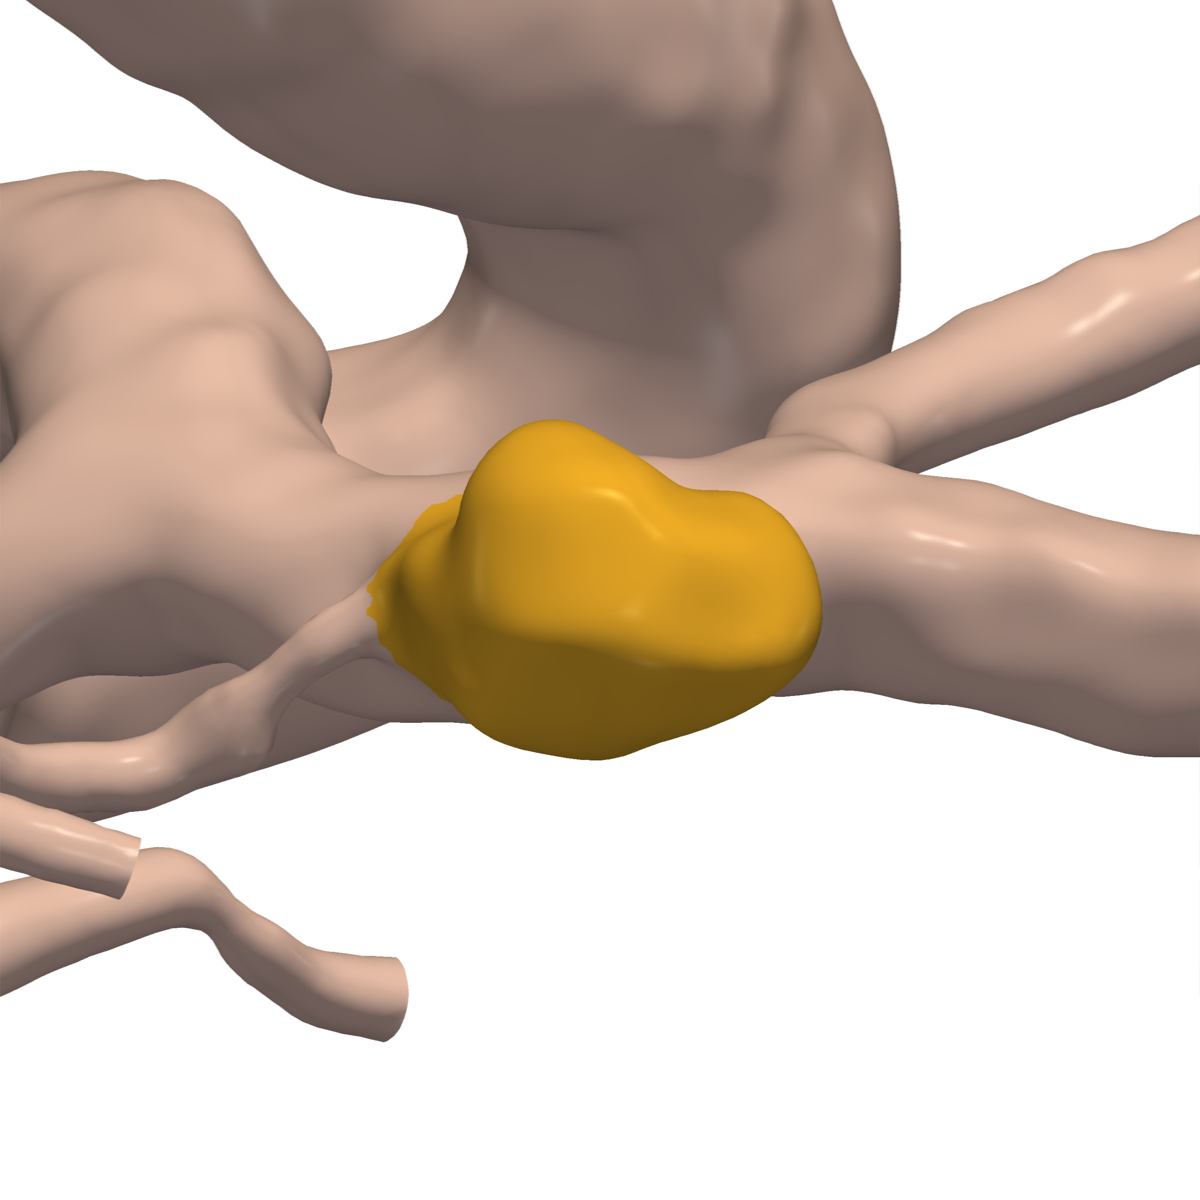
\includegraphics[width=0.325\textwidth]{figures/tmA_gt.png}\hfill
    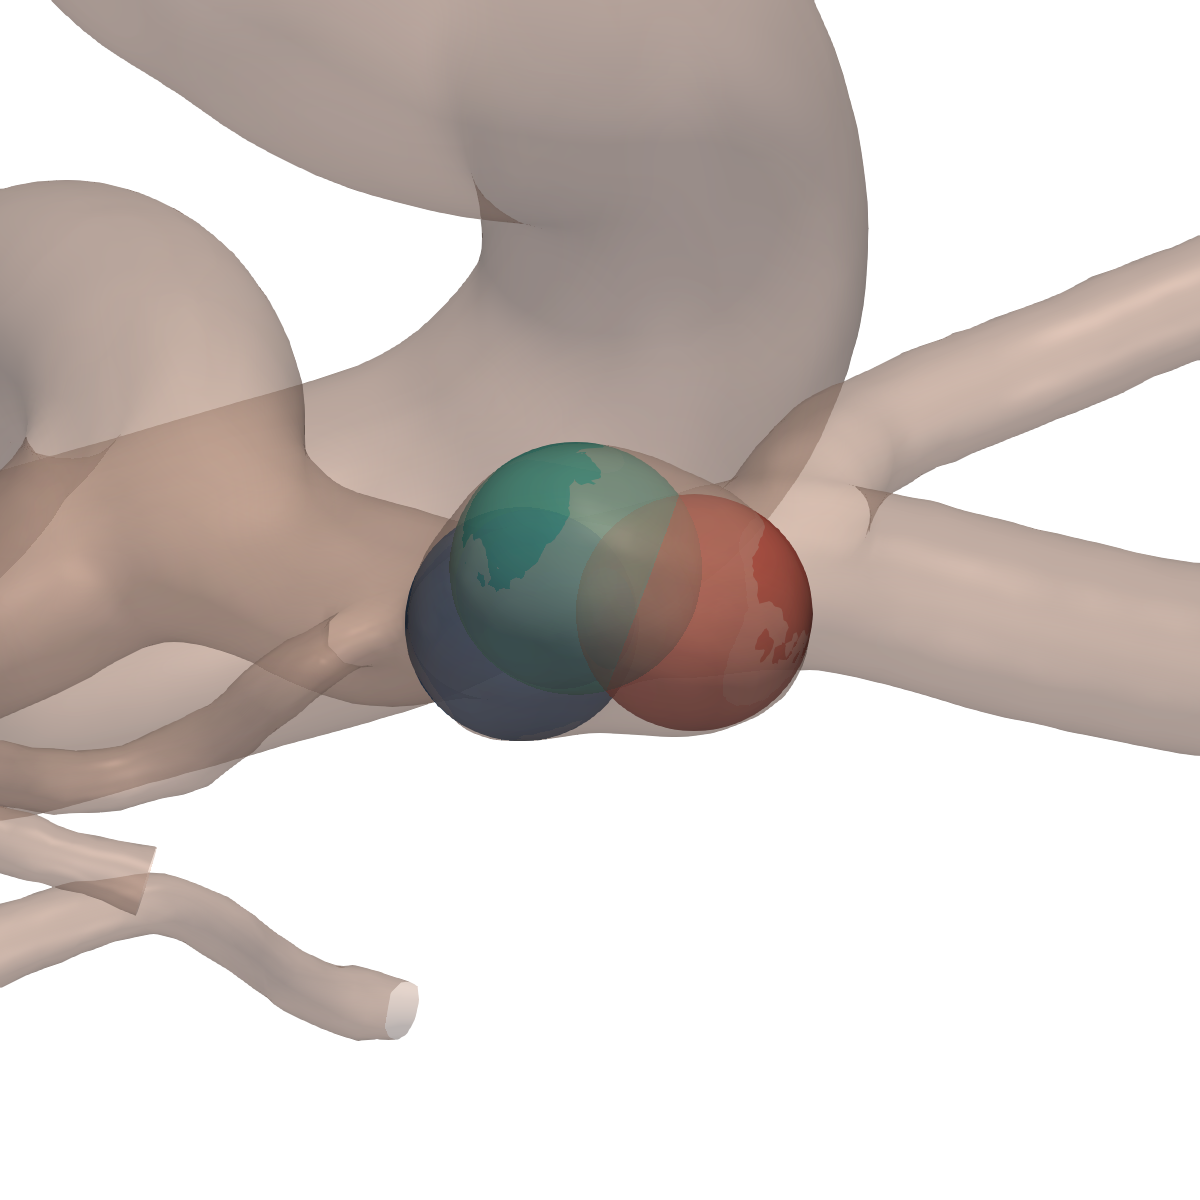
\includegraphics[width=0.325\textwidth]{figures/tmA_sph.png}\hfill
    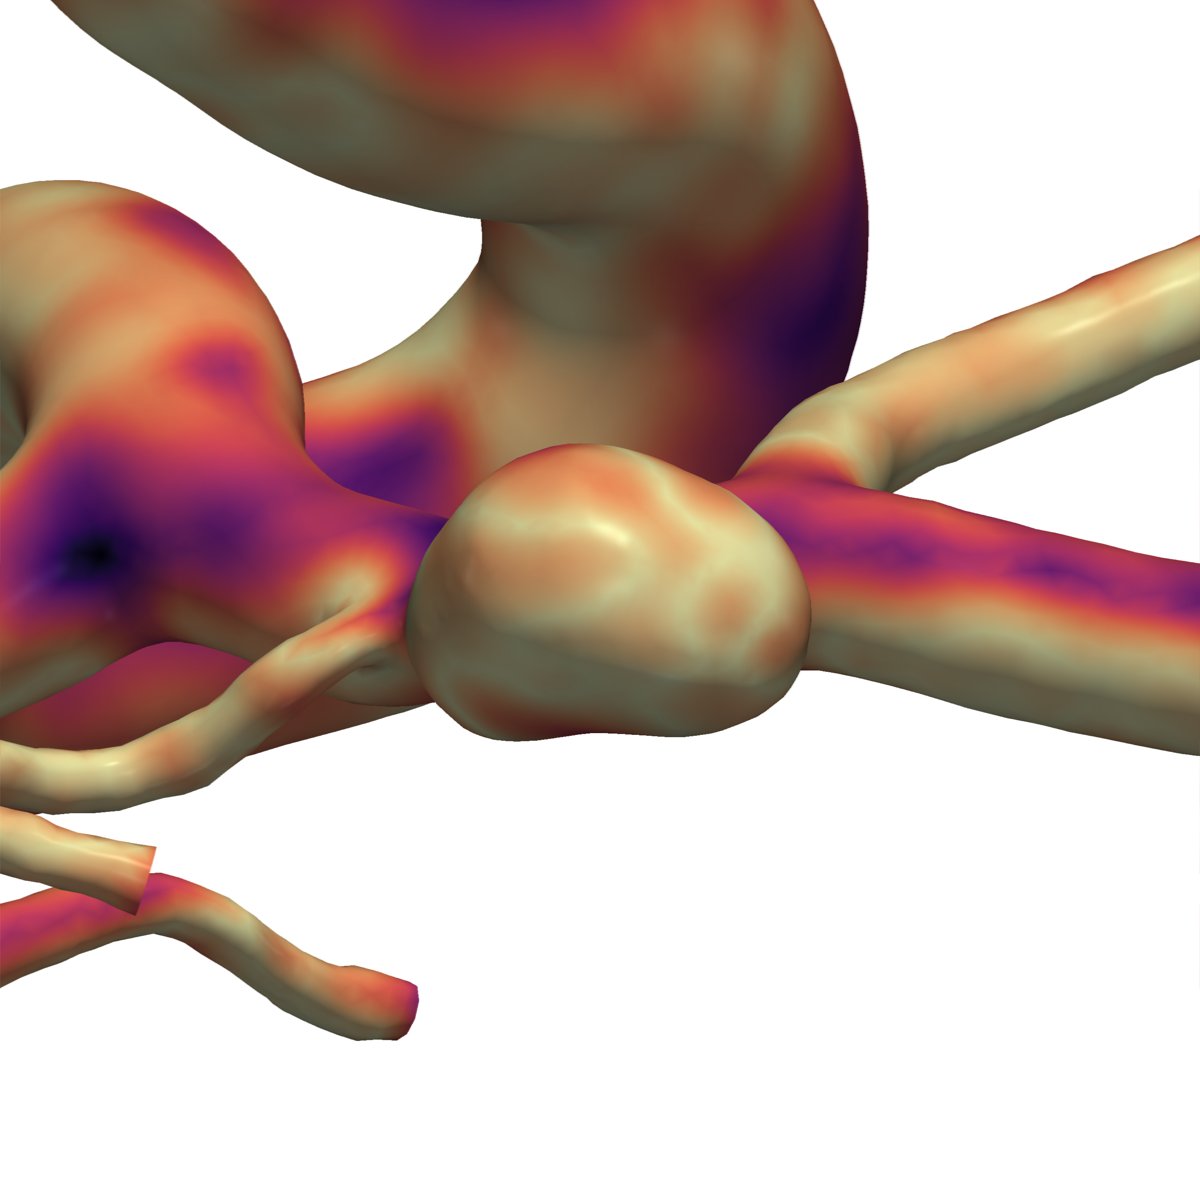
\includegraphics[width=0.325\textwidth]{figures/tmA_dist.png}\\[1mm]
    \hfill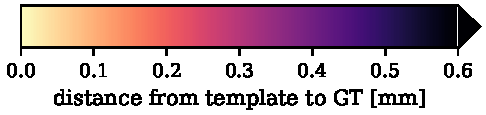
\includegraphics[width=0.325\textwidth]{figures/cbar_dist_06.pdf}
    \caption{Template creation on the example vessel. Left: the GT with the detected aneurysm (sac and neck lip) in yellow. Middle: the template (translucent) with the three fitted spheres. Right: the finished template, smoothed, meshed and cut at the ostia, coloured by the distance of each of its vertices to the GT surface. The scale ends at 0.6\,mm and saturates above it. Cream is below 0.1\,mm. On the sac the median distance is 0.06\,mm and the 95th percentile 0.20\,mm. On the parent it is larger (up to 0.9\,mm), since the 5\,mm radius knots deliberately ignore local calibre changes, which the network learns in the second stage.}
    \label{fig:dp_template}
\end{figure}

For the example vessel the fitted spheres have radii of 1.07, 1.16 and 1.09\,mm, and the template has 23\,052 vertices against the GT's 91\,395. We measure the distance from every vertex of the finished template to the nearest point of the GT surface. Over the whole template it has a median of 0.12\,mm and a 95th percentile of 0.42\,mm. On the sac alone the median is 0.06\,mm and the 95th percentile 0.20\,mm. Measured the other way, from the GT vertices to the template, which also sees sac wall that the template does not reach, the figures on the sac are 0.07 and 0.23\,mm. The largest deviations lie on the parent artery, where the 5\,mm radius knots deliberately ignore local bulges (Figure~\ref{fig:dp_template}). Across the dataset, a median of 5.9\% of the GT wall was detected as aneurysm, and the fitted sphere radii have a median of 1.58\,mm (5--95\%: 0.68--3.96\,mm).

Three spheres are a coarse description, and they fit the sac closely only when the sac is roughly round. Over the dataset, the median per-case median distance of the sac wall to the template is 0.13\,mm. In 10\% of the cases the median exceeds 0.30\,mm, and in 11 cases (1.5\%) it exceeds 0.5\,mm. The worst cases are giant sacs with calibres of several millimetres, and sacs that are elongated, flattened or multi-lobed, which three spheres of a common smooth minimum cannot follow. Figure~\ref{fig:dp_template_limit} shows one of them. The sac is a tall, tilted horn. The sphere penalty keeps every sphere inside the GT wall, so the fit settles on two large spheres stacked along the long axis and a small one near the tip, and the broad face of the sac sits up to 2--3\,mm outside the template. The sac surface of the template lies a median of 0.66\,mm from the GT wall (95th percentile 2.6\,mm, maximum 4.3\,mm), and the GT wall lies a median of 0.61\,mm from the template (95th percentile 1.95\,mm). We accept this, since the template is only the starting point of the second stage, but it also means that the network has to learn the shape of such sacs from the deformation, not from the template.

\begin{figure}[H]
    \centering
    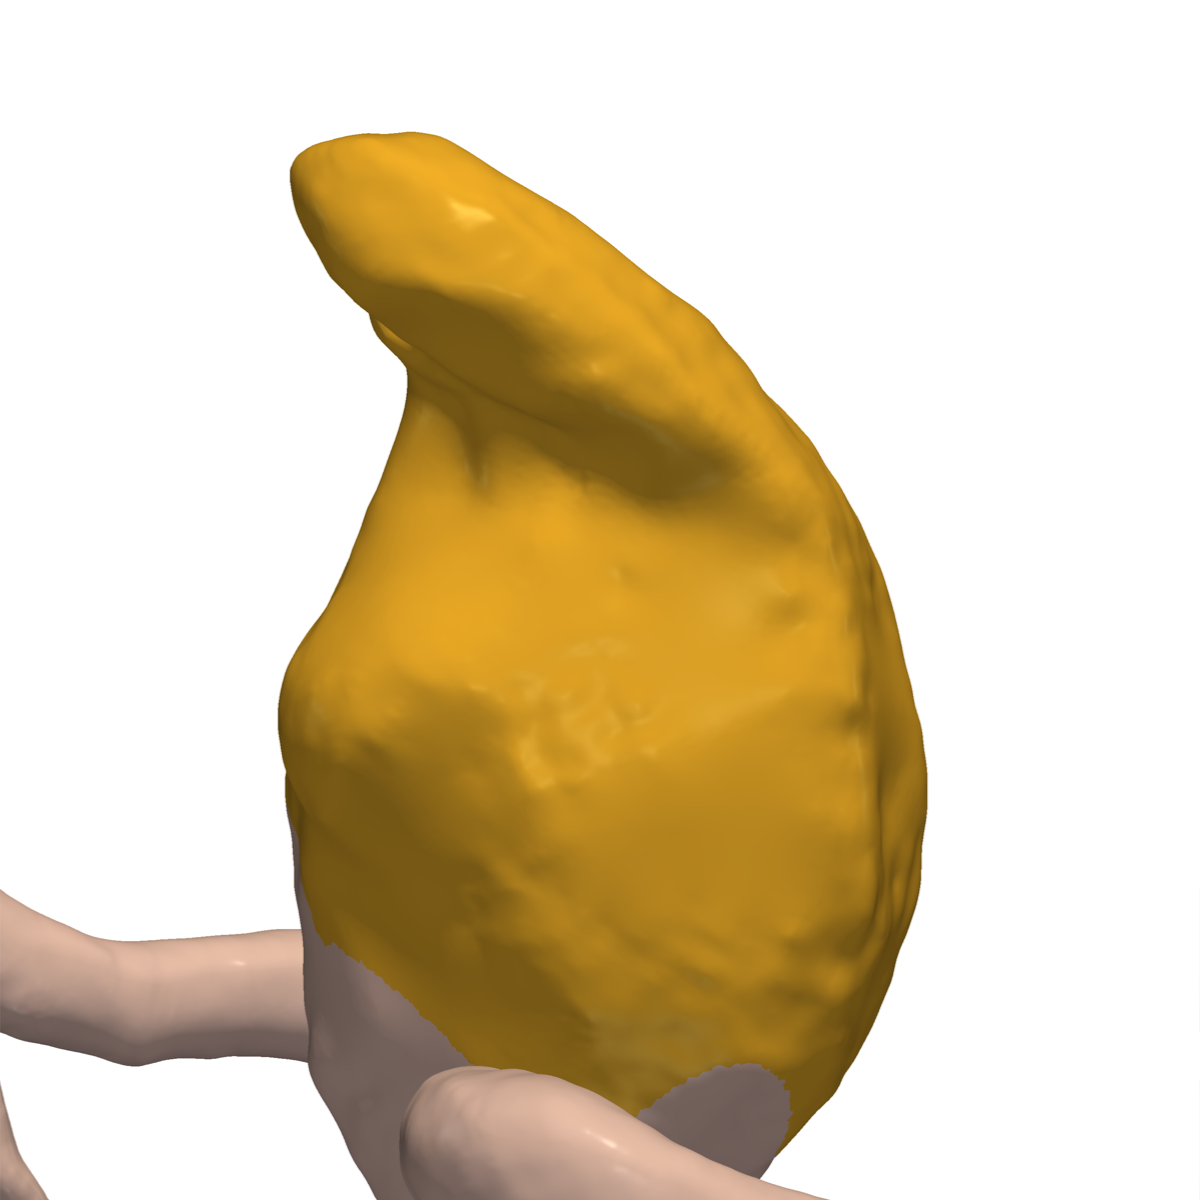
\includegraphics[width=0.325\textwidth]{figures/tmB_gt.png}\hfill
    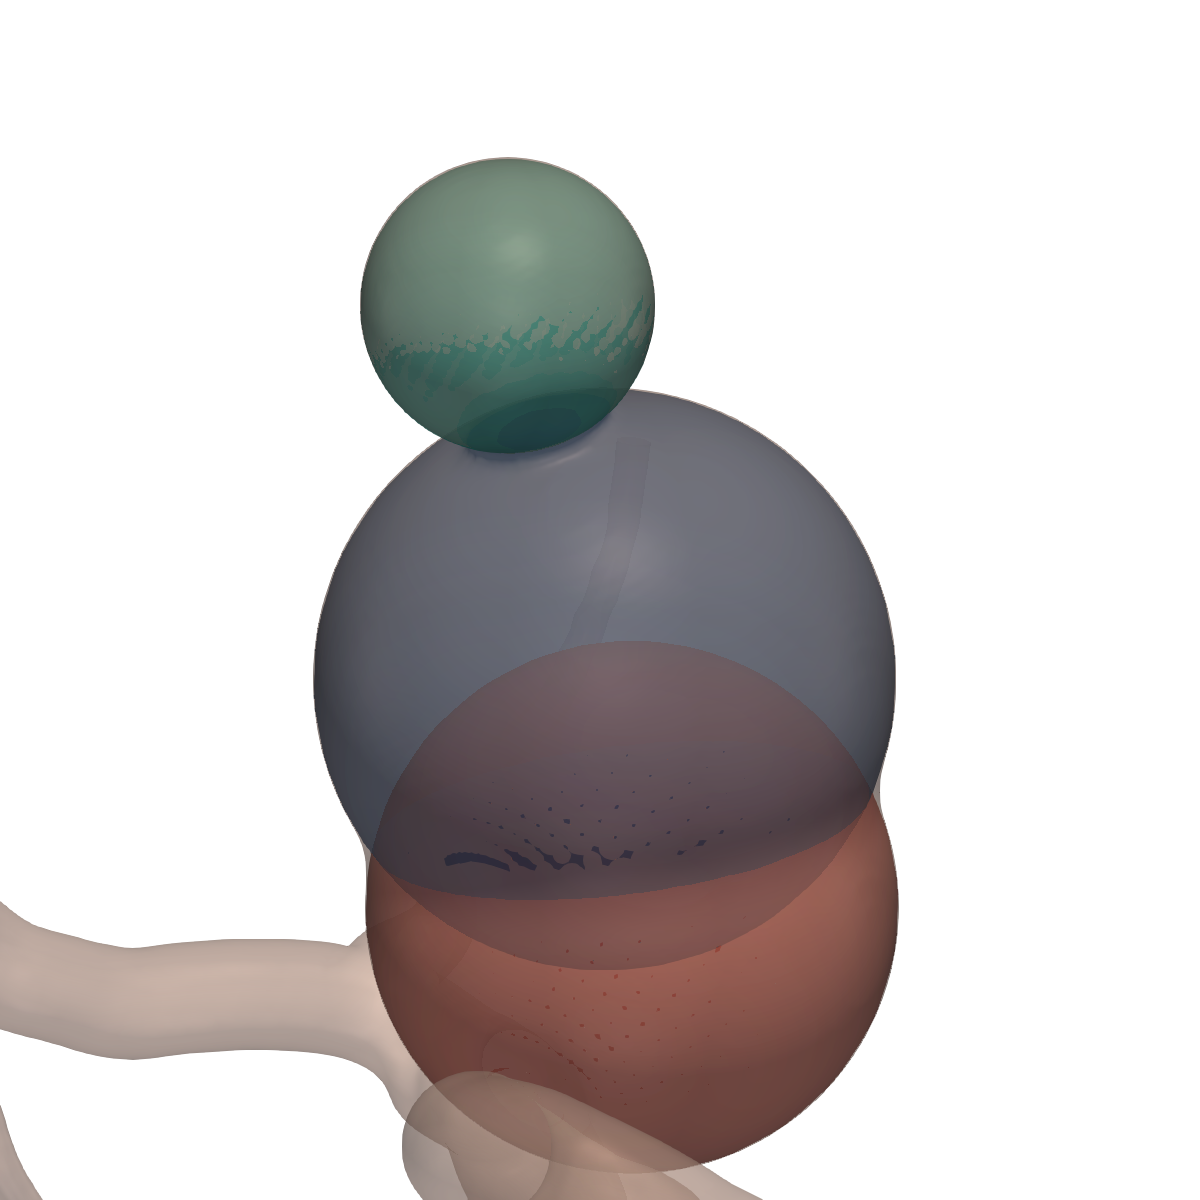
\includegraphics[width=0.325\textwidth]{figures/tmB_sph.png}\hfill
    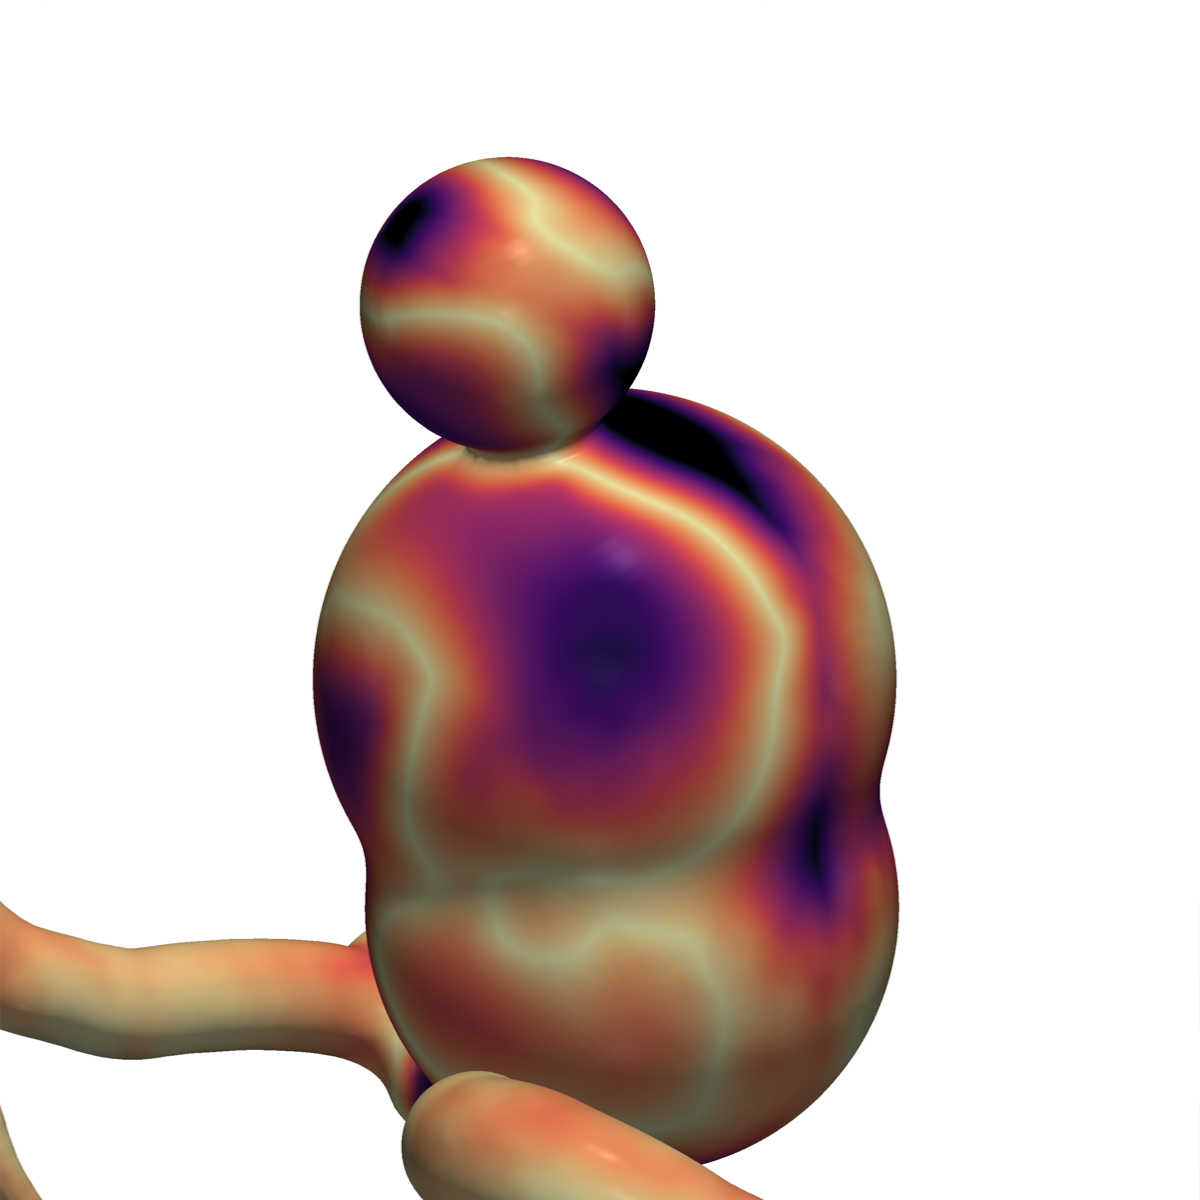
\includegraphics[width=0.325\textwidth]{figures/tmB_dist.png}\\[1mm]
    \hfill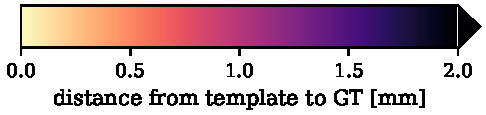
\includegraphics[width=0.325\textwidth]{figures/cbar_dist_20.pdf}
    \caption{A sac that three spheres cannot approximate. Left: the GT with the detected sac in yellow. Middle: the template with the three fitted spheres (radii 8.3, 4.2 and 7.6\,mm). Right: the finished template coloured by its distance to the GT, on a scale that ends at 2\,mm. The elongated, tilted sac is outside the spheres over most of its broad face and at its tip, and the spheres themselves bulge away from the wall between the rings where they touch it.}
    \label{fig:dp_template_limit}
\end{figure}


\subsection{Summary}
\label{sec:dp_summary}

Table~\ref{tab:dp_summary} summarises the pipeline. From 682 published vessel models it produces 737 training samples. Each consists of a single-aneurysm GT surface with a uniform 0.15\,mm triangulation and pipe-section openings, the ostium frames of those openings, a centreline with its inscribed radius, and a template built only from the centreline, the frames and three spheres. The two manual steps, cap removal and seed picking, are confined to the beginning of the pipeline. Everything after them is automatic, deterministic and gated, so the whole dataset can be regenerated from the published database whenever a stage changes.

\begin{table}[H]
    \centering
    \footnotesize
    \caption{Summary of the data-preparation stages.}
    \label{tab:dp_summary}
    \renewcommand{\arraystretch}{1.25}
    \begin{tabular}{p{3.0cm} p{3.6cm} p{4.6cm} p{2.6cm}}
        \hline
        \textbf{Stage} & \textbf{Input $\rightarrow$ output} & \textbf{Key method and parameters} & \textbf{Result} \\
        \hline
        Cap removal & 102 capped vessels & manual, Blender & 102 open \\
        Extension removal & 316 extended vessels & ring-wise cylinder test, $L \ge \max(1.5\,\text{mm}, 2R)$; local planar cut, $0.8$\,mm cuff & 2388 cuts \\
        Aneurysm isolation & 54 multi-aneurysm vessels & Voronoi parent reconstruction, graft onto original wall, gated retries & 117 samples \\
        Assembly & all of the above & priority merge, same-patient deduplication & 737 surfaces \\
        Uniform remeshing & 737 $\rightarrow$ 737 & pipe-section openings, isotropic remesh at 0.15\,mm & 737 GT + frames \\
        Centreline & 737 $\rightarrow$ 737 & Voronoi centreline, 0.1\,mm spacing, MISR, clipped at frames & 737 centrelines \\
        Template & 737 $\rightarrow$ 737 & parent tube (5\,mm knots) $\cup$ 3 fitted spheres, 0.3/0.15\,mm mesh & 737 templates \\
        \hline
    \end{tabular}
\end{table}
